\documentclass[11pt]{ociamthesis}  % default square logo 
%\documentclass[12pt,beltcrest]{ociamthesis} % use old belt crest logo
%\documentclass[12pt,shieldcrest]{ociamthesis} % use older shield crest logo

%load any additional packages
\usepackage{amssymb}
\usepackage{graphicx}
\usepackage{wrapfig}
\usepackage{parskip}
\usepackage{multicol}
\usepackage{titlesec}
\usepackage{setspace}
\usepackage{amsmath}
\usepackage[margin=20 mm]{geometry}
\usepackage{hyperref}
\usepackage{url}
\usepackage{amsmath,amssymb}
\usepackage{subcaption}
\doublespacing
\usepackage{csquotes}
\usepackage{longtable}
\usepackage{minted}
\usepackage{subcaption}
%\usepackage[inkscapelatex=false]{svg}
\hyphenpenalty = 1000
\usepackage{graphicx}
\graphicspath{ {figures/} }
\usepackage{array}
\usepackage{tikz} 
\usepackage{booktabs}
\usepackage[export]{adjustbox}
\usepackage{makecell}
\usepackage{array}
\usepackage{multirow}
%\usepackage{subfig}      
\usepackage{caption} 
\usepackage{subcaption}
\usepackage{titlesec}
\usepackage{enumitem}
\usepackage[font=small]{caption}
\usepackage{natbib}
\usepackage[acronym, toc, nonumberlist, nowarn, section]{glossaries}
\makeglossaries
% --- Acronyms ------------------------------------------------------
\newacronym{auam}{AuAM}{Auxiliary Attention Module}
\newacronym{cbam}{CBAM}{Convolutional Block Attention Module}
\newacronym{cbl}{CBL}{Convolutional Batch-Normalisation LeakyReLU}
\newacronym{cbr}{CBR}{Convolutional Batch-Normalisation ReLU}
\newacronym{ccd}{CCD}{Charge-Coupled Device}
\newacronym{cctv}{CCTV}{Closed-Circuit Television}
\newacronym{cnn}{CNN}{Convolutional Neural Network}
\newacronym{daf}{DAF}{Dilated Activation Function}
\newacronym{drdb}{DRDB}{Dilated Residual Dense Block}
\newacronym{ema}{EMA}{Exponential Moving Average}
\newacronym{estnet}{EstNet}{Rain‐Estimation Network}
\newacronym{gan}{GAN}{Generative Adversarial Network}
\newacronym{gpu}{GPU}{Graphics Processing Unit}
\newacronym{iso}{ISO}{Camera Sensor-Sensitivity Index (International Organization for Standardization)}
\newacronym{mca}{MCA}{Morphological Component Analysis}
\newacronym{mae}{MAE}{Mean Absolute Error}
\newacronym{mit}{MiT}{Mix Transformer}
\newacronym{mlp}{MLP}{Multi-Layer Perceptron}
\newacronym{mse}{MSE}{Mean Squared Error}
\newacronym{nlp}{NLP}{Natural Language Processing}
\newacronym{opm}{OPM}{Overlapped Patch Merging}
\newacronym{ords}{ORDS}{Oxford Rain Dataset}
\newacronym{pfr}{PFR}{Pyramid Feature Refinement}
\newacronym{psnr}{PSNR}{Peak Signal-to-Noise Ratio}
\newacronym{rcbam}{RCBAM}{Residual Convolutional Block Attention Module}
\newacronym{rcf}{RCF}{Richer Convolutional Features}
\newacronym{rcsa}{RCSA}{Residual Channel–Spatial Attention}
\newacronym{roi}{ROI}{Region of Interest}
\newacronym{segformer}{SegFormer}{Segmenter-Former Transformer Backbone}
\newacronym{ssim}{SSIM}{Structural Similarity Index Metric}
\newacronym{stb}{STB}{Sparse Transformer Block}
\newacronym{tsa}{TSA}{Top-$k$ Sparse Attention}
\newacronym{ugsst}{UGSST}{Uncertainty-Guided Semantic Segmentation Transformer}
\newacronym{unet}{U-Net}{U-Shaped Convolutional Network}
\newacronym{ustn}{USTN}{Uncertainty-Aware Sparse Transformer Network}
\newacronym{vit}{ViT}{Vision Transformer}

\titlespacing*{\section}   {0pt}{0.05\baselineskip}{0.05\baselineskip}
\titlespacing*{\subsection}{0pt}{0.05\baselineskip}{0.05\baselineskip}
\setlength{\parindent}{1.0em}  % indent first line
\setlength{\parskip}{0.1em} 
\doublespacing


%input macros (i.e. write your own macros file called mymacros.tex 
%and uncomment the next line)
%\include{mymacros}

\title{Removing Raindrops from Images Using Deep Learning}     % thesis title, 

\author{Mayowa Oyeleke}             %your name
\college{Lady Margaret Hall}  %your college

%\renewcommand{\submittedtext}{change the default text here if needed}
\supervisors{ Supervised by \\
                Professor Mauricio Villarroel \& Dr Shaun Davidson}
\degree{Master of Engineering}     %the degree
\degreedate{Trinity 2025}         %the degree date


%end the preamble and start the document
\begin{document}
\raggedbottom

\maketitle                  % create a title page from the preamble info
\include{dedication}        % include a dedication.tex file
\include{acknowlegements}   % include an acknowledgements.tex file
\begin{abstract}
    
Raindrops adhering to a camera lens blur texture, distort colour and thwart downstream computer-vision tasks that underpin autonomous driving, sports analytics and surveillance. This project aims to develop methods to remove raindrops from an image by utilising the power of deep learning models. The models explored have two main parts, a raindrop mask generating network, which identifies the regions in an image where raindrops are present, and a raindrop removal network, which recovers a raindrop free image. Extensive datasets are needed to train the deep learning models effectively. So a main part of the project was the collection of data from various environments and conditions where raindrops could adhere to camera lenses. In total, 320 images were captured, with 80 different backgrounds, each background consisting of 4 images, a clean image, and 3 varying levels of raindrop degradation. The state-of-the-art model is also recreated (model 1) with a novel introduction into the training process. To compare, the original state-of-the-art is also retrained and retested (model 2). A final model with the same underlying architecture, but that wasn't trained in an end-to-end fashion is also used as a benchmark for comparison (model 3). The quantitative metrics used to evaluate these models are the average peak signal to noise ratio (PSNR in dB), average structural similarity index metric (SSIM). All models achieve their maximum results on test set A, where model 1 achieves 27.1950 dB/0.8666, and models 2 and 3 achieve 26.3685 dB/0.8307, and 25.8567/0.8495, respectively. The novel implementation of the state-of-the-art allows it to outperform the other iterations of the model. The proposed novel model uses the same framework, with a mask generation network and a rain removal network. The mask generation network leverages semantic segmentation with uncertainty to create a mask generator robust to noise and uncertainty. My proposed novel model in the paper achieves results of 26.4808/0.8605. My novel model outperforms the original state-of-the-art when benchmarked on the same training and test set, and is only outperformed by the modified state-of-the-art from my contributions. 

\end{abstract}          % include the abstract

\begin{romanpages}          % start roman page numbering
\tableofcontents            % generate and include a table of contents
\listoffigures              % generate and include a list of figures

\begin{alwayssingle}
    \printglossary[type =\acronymtype, title ={List of Acronyms}]
\end{alwayssingle}

\end{romanpages}            % end roman page numbering


\chapter{Introduction}

\section{Motivation}

\label{Section:Motivation}
The increasing reliance on digital image processing across industries such as autonomous vehicle navigation, surveillance, sports technology, and other safety-critical applications has made the removal of rain-induced distortions from images an important area of research. Rain can obscure critical details in autonomous vehicle navigation \cite{article}, potentially leading to compromised navigation and object detection. CCTV cameras deployed for security can suffer from reduced visibility due to raindrops, leading to degraded footage quality, which poses risks in monitoring environments like incorrect object detection\cite{jia2012two}. Similarly, in sports technology like Hawkeye systems\cite{singh2012hawk}, rain-affected visuals can hinder accuracy impacting integrity of match analysis and decision-making. Addressing the potential for rain degradation to negatively impact object identification and decision making in these areas is vital for achieving reliable performance. 

The visual challenges introduced by rain are multifaceted, including rain mist, rain streaks, and raindrops, each of which affect image quality in distinct ways. Rain degradation on images is usually a combination of at least two of these. Images degraded with raindrops are particularly challenging to address due to the raindrops' tendency to blur, distort, obstruct fine details, and cause colour shifts in captured images. This is due to the raindrops' irregular shapes, closeness to image sensors and their long temporal presence in captured image frames \cite{hamzeh2021review}. Garg et al. \cite{1315077} studied the relation of a stationary raindrop to the radiance distribution of the environment and found that each raindrop behaves like a transparent sphere, refracting and reflecting light from the environment towards the camera. In addition, due to the finite exposure time of the camera, intensities of the image pixels due to rain are motion blurred and therefore depend on the background. \cite{1315077} states that raindrops attenuate about 6\% of the light refracted towards the camera and that the specular and internal reflections further add to the brightness of the drop. Thus, a drop tends to be much brighter than its background. This is an effect that is exploited in multiple papers to separate raindrops from the background (parts that the raindrop occludes). These effects mentioned lead to a significant loss of background image pixel information making it difficult for standard image restoration models to reconstruct rain-free images. In order to overcome these obstacles, there is a need for deep learning models capable of detecting and removing diverse rain patterns while accounting for real-world complexities and variations in raindrop sizes, densities, and impact angles.

The aim of this project is to develop a state-of-the-art model for the de-raining of images, specifically images degraded with raindrops, and to recreate and improve on the best-performing existing models. This project aims to build on the work done by Parmeet Singh Madan\cite{Parmeet_Report} in the 23/24  academic year in the Department of Engineering, and extend his methodologies in assembling a dataset and developing a novel model that is able to outperform the current state-of-the-art.




\section{Current methods}
\label{Section: Current Methods}
The field of rain removal is an active area of research with a number of research papers in the last decade. There are more studies on the removal of rain streaks from images, due to this being less challenging than raindrop removal because rain streaks predominantly have the same shape on images. There is also less literature on single image raindrop removal, with more papers focusing on temporal or sequential image tasks. This is due to the temporal information available in videos offering valuable image information for the reconstruction of the rain-free image. There are many traditional methods for raindrop removal from a single image in literature, for example involving the use of filters in \cite{6738189} where they use non-local means filtering on the detected rain areas by selecting non-local neighbour pixels and their weights adaptively. Other papers take advantage of the phenomenon that regions in an image obstructed by raindrops have a higher frequency than the unobstructed regions, mentioned in section \ref{Section:Motivation} and decompose the image into the low-frequency and high frequency parts using a bilateral filter. The high frequency part can then be decomposed into a "rain component" and a "non-rain component" via dictionary learning and sparse coding. The rain component can then be successfully removed from the image while preserving most original image details\cite{5946766}. Kanthan et al.\cite{7435707} also proposed a novel hybrid algorithm in order to detect raindrops, remove them and restore the image background in a single image. This hybrid algorithm is based on K-Means clustering and median filtering. Where K-Means clustering is used to classify the separate regions of the image, and eventually a median filter applied across the image to remove the raindrop pixels by taking the average over the neighbouring pixels. These traditional model-based methods cannot take advantage of the deep feature information of the image and find it hard to fully recover the comprehensive structural texture and edge knowledge, as well as the fine-grained raindrop shapes contained\cite{SHAO2021265}.


Convolutional neural network (CNN) based deep learning methods have shown better potential for this task in recent years due to their significantly representation capability to describe both raindrop shapes, and object textures/edges possibly occluded in the background. Some deep learning architectures have been specifically designed along this research line recently and have began to inspire the research trend for tackling this problem. Eigen et al.\cite{eigen2013restoring} was one of the first to apply a simple multilayer convolutional network to remove raindrops. Their neural network consisted of 3 layers of convolution with 512 neurons per layer, followed by a hyperbolic tangent activation function. This method worked, but was unable to provide clean results for large and dense raindrops. Moreover, the output images were somewhat blurred. The paper by Shao et al.\cite{SHAO2021265}, one of the more recent literature using CNNs for the task of raindrop removal from a single image, they propose a selective skip connection GAN (SSCGAN), combining the selective skip connection and self-attention mechanism to restore a clean image from a raindrop degraded one. Their methods combine the raindrop shape features with the background structure features to guide the network to accurately remove raindrops. Intrinsically, the key, and the most significant problem, for handling raindrop removal is how to encode the diverse and fine-grained raindrop shapes, and the complex and relatively more coarse-grained object structures, especially those occluded by raindrops, in the network architecture (for current deep learning methods). Therefore, current methods have room to be further improved to more sufficiently and elaborately deliver useful knowledge underlying both raindrops and background object structures \cite{SHAO2021265}. We will further explore in more detail, how some of the traditional and deep learning methods work in chapter \ref{Section:Literature Review}, the literature review section of this report.


\section{Objectives}

The main objectives for this project as follows:

\begin{enumerate}
    \item Extend the Oxford Rain Dataset (ORDS) with more real and varying raindrop corrupted data with their ground truths.
    \item Recreate the current state of the art model and analyse the model's performance.
    \item Introduce a novel framework building on the current state of the art models or otherwise.
\end{enumerate}

\section{Report outline}
This report will detail my research guided by the objectives above. I will conduct a literature review of previous methods that have been explored in this field. I will then detail the datasets available to me, and my protocol for collecting more data in order to aid in future research into this topic. I will also recreate a current state of the art model, assessing its performance on the chosen datasets, comparing to other models trained on the same dataset. Following this, I will propose a novel method, aiming to build on the limitations of the recreated state-of-the-art model and assess the performance of this model in comparison to other models trained on the same data. The final chapter will discuss the work in this report, and potential avenues for future work that can be explored.


\chapter{Literature review}
\label{Section:Literature Review}

\section{Introduction}
In this chapter, I will examine the contemporary approaches used in the literature for raindrop removal. This exploration will encompass both traditional image processing techniques and advanced deep learning methods that leverage data to train convolutional neural networks (CNNs) for effective raindrop removal. Due to the recent success of Transformers in Natural Language Processing (NLP), there has been a recent increase in interest in applying transformers to vision tasks. In order to keep up to date with the literature in this field of study, I will also include some of the research that has been done with transformers in the task of raindrop removal. All of these methods begin by pinpointing the locations of raindrops in the image. Subsequently, various techniques are applied to eliminate the raindrops, with the goal of creating a clear, rain-free image.

\section{Traditional methods}
One of the first to develop a raindrop removal method was Xu et al.\cite{xu2012improved}, where they aim to remove rain and snow by deriving a guidance image from the imaging model of a raindrop / snowflake when it passes through an element on the camera's charged-coupled device (CCD). The CCD is a light-sensitive integrated circuit that captures images by converting photons into electrons. The guidance image is computed based on the effect of raindrops captured by the camera, where the intensity of the pixels is a linear combination of the irradiance of raindrops and the irradiance of the background. Subtracting the minimum intensities from the maximum intensities gives a guidance image that is not affected by rain or snow. This means that the guidance image preserves the contours of the background image while eliminating any edges created by rain or snow. However, only using the guidance image led to the loss of some detailed information, as a result, the paper proposes a refined guidance image. The refined guidance image has contours similar to the undegraded image and also maintains detailed information that may be lost in the guidance image. A filtering method can then be used to remove the linear edges caused by rain or snow (in the paper a guided filter\cite{6319316} is used). The more well-known bilateral filter could also be used, but the guided filter has better behaviour near the edges, leading to less detailed information being lost. Quantitatively, the method was effective in removing the effects of snow and rain and worked better when a refined guidance image was used. The method retained some detailed information, but a qualitative inspection of the results shows that the output image is blurred, losing some of the information in the image. The method also performs worse when the scene is complex, especially when objects and backgrounds with similar appearances to rain or snow are present. 

The next traditional method was proposed by Fu et al.\cite{Fu5946766}, based on the idea that the lack of temporal information in a single image makes rain removal more challenging. Their method aims to mitigate this challenge, and they were among the first to propose a single frame-based rain removal framework by formulating the problem as an image decomposition problem based on Morphological Component Analysis (MCA)\cite{MCA10.1117/12.615237}. MCA separates features in an image with different morphological aspects. It can be used to decompose images into their texture and piecewise smooth parts, or for inpainting applications. Instead of directly applying conventional image decomposition techniques, they first decompose an image into high-frequency and low-frequency parts using a bilateral filter\cite{BilateralFiltering}. The high frequency part is then decomposed into the "rain component" and the "non-rain component" through dictionary learning and sparse coding\cite{DictionaryLearningForSparseCoding}\cite{SparseRepresentations}. As a result, no temporal or motion information is required between successive images. The most basic information is in the low-frequency parts, whereas the rain streaks and other edge/texture information will be included in the high-frequency part. After the high-frequency part is separated into rain and non-rain, training exemplars are extracted from the image itself in the dictionary learning stage. The paper uses the curvelet basis\cite{Curvelet} as a global dictionary to represent the geometric component of the high-frequency part. The rain patches from the high-frequency image were extracted as training exemplars. Based on the learned dictionary of the curvelet and rain dictionaries combined, they perform sparse coding via applying the Orthogonal Matching Pursuit (OMP)\cite{OMP} algorithm for each patch extracted from the high-frequency image via minimising to find its sparse cooefficients. Different from MCA, sparse coding is performed once for each patch with respect to the learned dictionary. Each reconstructed patch can then be used to recover either a geometric component or a rain component based on the sparse coefficient. The method was able to remove rain degradation to a good level without blurring the output image, it performed better than just using a bilateral filter or a MCA based approach. A significant drawback is that for colour images, the output of the model is a black and white image. Methods to predict the original colour present in the images could likely be employed to return the colour, but of course a method that doesn't remove the colour in the first place would be preferred.

The final traditional based method I will discuss is a paper from Wu et al.\cite{WuEtAl6467016} that focuses on removing raindrops on vehicle windshields. The approach is a novel method that detects and removed raindrops in the captured image using a single in-vehicle camera. It uses the assumption that in light or moderate rainy conditions, raindrops appear as small circles on the windshield. The method analyses the colour, texture and shape characteristics of raindrops in images, and through this they identify possible raindrop candidates in the Regions Of Interest (ROI), which are small locally salient droplets in a raindrop saliency map\cite{SaliencyMapenwiki:1276598565} to highlight the most relevant regions. They then propose a learning-based verification algorithm to reduce the number of false alarms (i.e clear regions mis-detected as raindrops). The regions occupied by raindrops are then filled in using image inpainting techniques, using the intensity information of neighbouring pixels. This is possible since the shape of a raindrop changes the local image intensity, making the raindrop exhibit local saliency. This is due to the property of raindrops having high intensity, because they accumulate light from multiple sources due to them acting like a lens, making them have a high contrast compared to their surrounding regions. An example of the proposed raindrop detection and removal is shown in figure \ref{Figure: Wu et al. Raindrop removal proposal}. The model worked well in conditions where the shape, colour and texture of the raindrops were evident, such as driving at high speed in moderate rain or at low speed under light rain. However, in situations where the camera was closer to the screen, meaning the raindrops were more blurred without much saliency, or in heavy rain where the shapes of the raindrops are more complicated, the assumptions of the model are violated and the model doesn't work well in these cases. This coupled with the fact that the method is limited to only images of the road, means the method is not robust and is not generalisable to other situations and environments.

\begin{figure}[h]
    \centering
    \includegraphics[width=0.8\textwidth]{figures/Wu et al Raindrop removal proposal.png}
    \caption{Example of raindrop detection and removal. (A) Original Image with ROI in the yellow rectangle. (B) Raindrop Candidates. (C) Raindrop Detection (Red dots signify raindrops chosen). (D) Clean image after raindrop removal } 
    \label{Figure: Wu et al. Raindrop removal proposal}
\end{figure}

\section{Deep learning methods}

In order to address the limitations of traditional raindrop removal techniques, researchers have increasingly turned to deep learning methods. These techniques leverage large datasets and powerful neural network architectures to learn features and patterns associated with raindrop presence and effects. These models can then use the information from the features and patterns learned to remove the raindrops and reconstruct a rain free image. Common architectures used in this endeavour include Convolutional Neural Networks (CNNs), and in more recent times, transformers. This section will examine some of the prominent deep learning approaches that have been applied to raindrop removal, highlighting their methodologies, effectiveness, and comparative advantages.

\subsection{Convolutional Neural Networks (CNNs)}

After the work done by Eigen et al.\cite{eigen2013restoring}, one of the first to apply a multi-layer network for the task of raindrop removal, discussed in section \ref{Section: Current Methods}, Qian et al\cite{qian2018attentive} was amongst the next papers to make further strides in the field of raindrop removal with CNNs. They apply an attentive generative network using adversarial training. The main idea was to inject attention\cite{bahdanau2014neural} into both the generative and discriminative networks, namely the generator and discriminator in AttGAN. During training, the visual attention learns about the raindrop regions and their surroundings. The attention map is trained by comparing it to a binary mask of the raindrop regions, using the mean squared error (MSE) loss function. By injecting this information, the generative network pays more attention to the raindrop regions and the surrounding structures, and the discriminative network will be able to assess the local consistency of the restored regions. The generative network is responsible for generating the attention map, which guides the autoencoder that reconstructs the raindrop-free image using contextual information. The discriminative network assesses whether the generated output is realistic by checking it globally and locally, and is also guided by the attention map, allowing it to focus on areas that may contain artefacts or inaccuracies. The model is trained using a Generative Adversarial Network (GAN)\cite{goodfellow2014generative}, which facilitates the creation of high-quality outputs through a competitive learning process. The authors of the paper also created a benchmark dataset with 1119 image pairs, each pair consisting of raindrop-covered and raindrop-free images of the same background. This was one of the main contributions of the paper. Their method also performed well, outperforming other start-of-the-art methods including Eigen et al.\cite{eigen2013restoring}, showing better image quality and fewer artefacts after restoration. Visual comparisons also show that AttGAN produced cleaner results with better restoration of background structures, particularly in cases with dense and large raindrops. However, AttGAN only utilizes the shape information of the raindrops, it does not utilize the texture information of the background structure. When the raindrops vary in the image, it is difficult to extract the complete raindrop shape features, so the output is blurred. The method is also highly dependent on the availability of high-quality raindrop masks that are used as ground truths for training the neural network. The masks used in this method are binary masks, which are acquired by subtracting the rain-free image from the rainy image, then setting a threshold value setting everything above the threshold to the max pixel value and everything below to 0. The paper proposes a dataset for training neural network based raindrop removers. However, the ground truth raindrop masks are not very accurate owing to several factors like the binarization of the mask leading to accuracy loss and the imperfect alignment of rainy image and raindrop-free image\cite{quan2019deep}.

Quan et al.\cite{quan2019deep} also propose a CNN for removing the effects of raindrops from an image. The proposed CNN introduces a double attention mechanism that concurrently guides the CNN using shape driven attention and channel re-calibration. The shape driven attention exploits physical shape priors of raindrops, like convexness and contour closedness, to accurately locate raindrops. This is implemented using a torque-based measure\cite{nishigaki2012image} that aligns with the properties of elliptical shapes of raindrops, helping focus attention on areas likely containing raindrops. This helps the model identify raindrop regions without relying on simplistic binary masks. The channel-recalibration improves the robustness when processing raindrops with varying appearances. This is because not all channels (features) are useful in the process of removing raindrops as some are more relevant to the raindrop layer. By recalibrating the channel-wise importance of these features, the network can focus on the most relevant features during restoration, leading to more accurate and artefact-free outputs. The network follows an encoder-decoder architecture with residual blocks. It also incorporates the joint physical shape + channel attention module within the residual blocks. The input image is first passed through a convolutional network to extract features, then the network's encoder decodes spatial patterns from the image while capturing the variations caused by the raindrops. The joint attention mechanism then helps the model focus on the relevant areas in the image. The encoder-decoder structure then processes the features, with the decoder reconstructing the image by progressively refining it. The attention modules assist by guiding the model's focus on the raindrop regions to ensure the removal process works effectively. The paper uses the dataset from Qian et al.\cite{qian2018attentive}, and comparison with other methods like Eigen et al.\cite{eigen2013restoring} and AttGAN\cite{qian2018attentive} shows an improvement in performance in terms of quantitative metrics, and the visual quality of the output images. A visualization of their results compared to Qian et al's is shown in figure \ref{Figure: Quan et al. 2019}. 

\begin{figure}[h]
    \centering
    \includegraphics[width=0.5\textwidth, height = 0.4\textwidth]{figures/Quan et al's results.png}
    \caption{Example of Quan et al's. and Qian et al's. performance on a raindrop degraded image } 
    \label{Figure: Quan et al. 2019}
\end{figure}

The final CNN-based method I will discuss is the paper by Kwon et al.\cite{Kwon}. The proposed model comprises a raindrop mask network and a raindrop removal network. The raindrop mask network is based on the U-Net architecture\cite{U-Net}, which learns the location, shape and brightness of raindrops. The raindrop removal network is a GAN also based on U-Net and comprises two attention modules, the raindrop mask module and the residual convolutional block attention module\cite{woo2018cbam}. The U-Net is a CNN architecture commonly used in image segmentation tasks. It consists of an encoder-decoder structure with skip connections that help preserve spatial information. In this paper, U-Net is employed for raindrop-mask generation. The mask generated is used by the subsequent raindrop removal network to focus on the affected areas. The advantage of the mask used in this paper over traditional binary masks lies in its ability to capture subtle intensity and size variations of raindrops, ensuring more precise raindrop identification. The generator in the raindrop removal network uses a combination of the raindrop image and the raindrop mask as inputs to produce a clean image. It also integrates the residual convolutional block attention module (RCBAM), which enhances the model's attention to raindrop affected areas. The generator outputs images at different resolutions, improving detail and restoration quality. The discriminator, based on PatchGAN\cite{PatchGAN} architecture, evaluates the generated images by distinguishing between real and generated image patches. This helps in ensuring more realistic restoration by focusing on local details. The proposed model outperforms current state-of-the-art models in terms of raindrop removal, with fewer artefacts and better preservation of image details., producing high quality results both qualitatively and quantitatively. This makes this the current state-of-the-art model and similar to \cite{Parmeet_Report}, I will recreate and assess the performance of this model later in this report. 

\subsection{Transformers}

CNNs are very powerful and are able to easily achieve better performance than prior hand crafted methods. One of the limitations of CNNs is that they have difficulty capturing long-range dependencies due to the limitations of convolution. This is because CNNs use convolutional kernels that slide across the input (An image for the purposes discussed in this paper), so they are only able to process the information in that small patch of the data. So, the kernel can learn local features and relationships within it, but it is difficult for a CNN to capture dependencies spanning a long distance in the input image. Deeper CNNs gradually build up longer range dependence as the receptive field increases with model depth, but increasing the depth also increases the complexity and size of the model. Transformers were first introduced by Vaswani et al.\cite{vaswani2017attention}, initially used in natural language processing (NLP) tasks. Their self-attention mechanism removed the need for sequential processing and allowed them to capture relationships across sequences in a highly parallel and efficient way in the encoder layer. This led to the emergence of Transformers as a dominant architecture in various domains beyond NLP, including computer vision and speech recognition. Where, similar to their design in NLP, the authors split an image into multiple linearly embedded patches, called tokens, which are then fed into a standard transformer alongside positional embeddings (PE), that provide the model with information about the position of each token within the image. Notably, Vision Transformers (ViTs), first introduced in \cite{dosovitskiy2020image}, leverage the self-attention mechanism to model global relationships in image data, thus overcoming the limitations of CNNs in capturing long-range dependencies. This shift has prompted researchers to explore the applicability of Transformer-based architectures across a spectrum of tasks, resulting in significant advances in both performance and versatility.

An example of a paper that utilises Transformer based architecture for raindrop removal in images is by Fu et al.\cite{fu2024uncertainty}. Raindrops often exhibit a unique sparse distribution in images, but current methods for removing raindrops apply a uniform treatment of pixels. Current approaches fail to measure the specific degradation within raindrop regions, such as variations in shape, size and transparency. Their paper proposes an Uncertainty-aware Sparse Transformer Network (USTN) to address these problems. To characterise the sparsity of raindrops, they develop a sparse transformer backbone in which several Sparse Transformers Blocks\cite{child2019generatinglongsequencessparse} (STBs) are deployed at each scale. To ensure effective sparse feature learning, they introduce a Top-k Sparse Attention (TSA) layer in each STB, which dynamically selects high score attention and generates corresponding sparse feature responses. To effectively model various degrees of degradation in local raindrop regions, they incorporate image uncertainty estimation, which can explicitly show the observation that worse degradation exhibits higher uncertainty. They design two decoding branches, one for estimating uncertainty maps and the other for generating raindrop-free images. Then they formulate an uncertainty-driven loss to better push the USTN to remove raindrops guided by uncertainty maps. In order to further refine the learned sparse features, they propose a Pyramid Feature Refinement (PFR) module to fully mine the local features under multiscale receptive fields and a Residual Channel-Spatial Attention (RCSA) module to stimulate the effective expression of the deepest features. All these components allow the USTN to produce high-quality results both qualitatively and quantitatively, preserving the details of the rain-degraded images. 



\chapter{Datasets}
\label{Chapter:Datasets}

As mentioned in the previous sections, the effectiveness of image de-raining models based on deep learning significantly rely on the quality and diversity of the datasets used for training and evaluation. This chapter covers the datasets employed in this project. My novel contributions include a collection protocol used to collect new data for this project and to aid in future research. 

\section{Existing datasets}

There are a number of datasets in the literature, including recent datasets gathered for the advancement of this same project title. These datasets have been used in various studies to benchmark the performance of different models in the field.

Qian et al.\cite{qian2018attentive} was the first to release a dataset containing rain-degraded images and their ground truth rain-free images. To obtain this data, they used two pieces of the same glass, one sprayed with water and the other clean. They managed any causes of misalignment, such as the movement of the camera, and ensured that the weather conditions (sunlight, clouds) and background objects were static during the image capturing. In total, they captured 1168 images, with varying backgrounds and raindrop degradations. Some examples of their captured images are in figure \ref{fig:qian_example}.

\begin{figure}[ht]
    \centering
    \includegraphics[width=0.8\textwidth, height=0.4\textheight, keepaspectratio]{figures/Qian et al dataset examples.png}
    \caption{Example images from the Qian et al. dataset.}
    \label{fig:qian_example}
\end{figure}

Another dataset used in the literature is named RainDS and was released by Quan et al.\cite{quan2021removing}. They collect a real-world rain dataset, which includes multiple image pairs in varying lighting conditions and scenes. Each image pair contains four images, a rain streak image, a raindrop image, an image with both rain streaks and raindrops, and finally the rain-free image. RainDS stands out from the previous dataset as they incorporate a synthetic subset of data. They generated the synthetic rainy data based on first person driving scenes collected from public autonomous driving datasets. They use a similar protocol to collect their real world images as Qian et al. In total there are 250 image pairs for the real-world images, and 1200 image pairs for the synthetic images. As there are four images per pair this leads to a total of 5800 images. Some examples of the images are in figure \ref{fig:quan_example}.

\begin{figure}[ht]
    \centering
    \includegraphics[width=0.8\textwidth, height=0.4\textheight, keepaspectratio]{figures/Quan(RainDS) dataset examples.png}
    \caption{Example images from Quan et al's. dataset with synthetic and real-world images}
    \label{fig:quan_example}
\end{figure}

The final dataset used in this paper was collected by Parmeet et al.\cite{Parmeet_Report} in the previous year. Building on the methods of Qian et al. and Quan et al., they established a robust and repeatable process for gathering data. Specifically, they captured images at different apertures and spraying distances to vary both the sharpness of the raindrops and the degree of raindrop degradation. Whenever they took a rain-degraded image using a glass slab, they would rotate the slab and capture another image, yielding two distinct raindrop patterns for each unique background. In total, they photographed 40 different locations under multiple aperture and spraying-distance settings, resulting in 80 images for every specific combination of these parameters. The apertures used were f/4, f/8, f/16, and f/22, while the spray distances were 30 cm, 50 cm, and 70 cm. Any combination of aperture and spraying distance can therefore be selected from this dataset. A snippet of the collected data in this paper is present in figure \ref{fig:rainy_small}.

\subsection{Current dataset splits}
Parmeet et al.\cite{Parmeet_Report} analysed the two datasets mentioned above and created  3 unique datasets by combining them in certain ways. The datasets are split via the standard 80-20 (training-test) split, and the training data is split into training and validation data using the training strategy that will be detailed in the subsequent chapters. An overview of these datasets are shown below.

\textbf{Dataset A} - Real data from Qian et al.\cite{qian2018attentive}.
\begin{table}[ht]
    \centering
    \begin{tabular}{@{}l r@{}}
        \toprule
        Dataset & Overall Training Set (80\% of all real data) \\
        \midrule
        Qian et al. & 934 \\
        \bottomrule
    \end{tabular}
    \caption{Summary of Dataset A containing the real data from Qian et al.}
    \label{table:dataset_a}
\end{table}


\textbf{Dataset B} - Real data from Qian et al. and Quan et al.\cite{quan2021removing}.
\begin{table}[ht]
    \centering
    \begin{tabular}{@{}l r@{}}
        \toprule
        Dataset & Overall Training Set (80\% of all real data) \\
        \midrule
        Qian et al. & 934 \\
        Quan et al. & 174 \\
        \midrule
        Total & 1108 \\
        \bottomrule
    \end{tabular}
    \caption{Summary of Dataset B.}
    \label{table:dataset_b}
\end{table}

\textbf{Dataset C} - Real data from Qian et al. and Quan et al. All the synthetic data from Quan et al. 
\begin{table}[ht]
    \centering
    \begin{tabular}{@{}l c c@{}}
        \toprule
        Dataset & \multicolumn{2}{c}{Overall Training Set} \\
        \cmidrule(lr){2-3}
                  & Real-80\% & Synthetic-100\% \\
        \midrule
        Qian et al. & 934  & --   \\
        Quan et al. & 174  & 1125 \\
        \midrule
        Total & 1108 & 1125 \\
        \midrule
        Overall Total & \multicolumn{2}{c}{2233} \\
        \bottomrule
    \end{tabular}
    \caption{Summary of Dataset C.}
    \label{table:dataset_c}
\end{table}

Two test sets are created to assess the performance of these models on unseen data from the two datasets above, with a third test set included from the ORDS collected by Parmeet et al.\cite{Parmeet_Report} in the previous year of this project. The combination of aperture and spraying distance chosen is f/16 and 50cm.

\textbf{Test sets} - The test sets used to evaluate the performance of the models.
\begin{table}[h!]
    \centering
    \begin{tabular}{@{}lccc@{}}
        \toprule
        Dataset & Test Set A & Test Set B & Test Set C \\
        \midrule
        Qian et al & 234 & -- & -- \\
        Quan et al & -- & 44 & -- \\
        ORDS       & -- & -- & 80 \\
        \bottomrule
    \end{tabular}
    \caption{Summary of Test Sets.}
    \label{table:test_sets}
\end{table}

Dataset C is the largest and most diverse dataset, as it integrates both real and synthetic data. In light of its breadth and variability, the models developed in this paper are trained using Dataset C.

\subsection{Data augmentation}
In order to bring all the images to the same size for training simplicity, and also increase the dataset size, Parmeet et al.\cite{Parmeet_Report} apply data augmentation to the dataset. Smaller images of size $256 \times 256$ are first obtained from the image. The images were further enhanced by flipping the images, horizontally or vertically, or keeping the image unchanged, each with a chance of $1 \over 3$. Using this process, dataset C with a total size of $2233$ images total, is increased to $16971$ images. With the training set from Qian et al. increasing from $934$ images to $5889$ images, the real training set from Quan et al. went from $174$ images to $3132$ images, and the synthetic training set from Quan et al. increasing from $1125$ images to $7950$ images, allowing for a larger training set than otherwise. Note that the images in test sets A and B are also augmented, so are the same size as the images in the training set, the images in test set C are not augmented.

\section{Data collection}

The first objective for this project was to extend the current Oxford Rain Dataset (ORDS) with more real and varying raindrop data. This was an objective for the following reasons:

\begin{itemize}
    \item Implement a data collection protocol that can be repeated by future studies to aid in the collection of new datasets.
    \item Create new benchmark train/test sets for future studies to assess the performance of models on.
    \item To test the models created in this paper against the benchmark test sets to assess performance.
    \item To enhance the diversity and robustness of the training data, which is crucial for model generalization in real-world scenarios.
\end{itemize}

I will now outline the data collection method I used and the different factors that I considered throughout the process.

\subsection{Parameters of interest}

Multiple parameters need to be considered when capturing images, for example the ISO, which refers to the sensitivity of the camera sensor to light. Higher values of ISO mean the sensor is more sensitive and images are brighter, so it is better for lower light conditions and vice versa for lower ISO values. This parameter was fixed at 64 and kept constant for all images.

Another parameter of interest was the aperture. This refers to the size of the opening in the lens that allows light to pass through to the sensor. The aperture is measured in f-stops, and the lower the f-stop, the larger the opening and the more light that is let in. Aperture affects the range between the nearest and furthest objects in focus in an image. A narrow aperture will result in a greater depth of field, and a larger aperture will produce a shallower depth of field. A higher f-stop number corresponds to a narrower aperture which lets in less light. As a narrow aperture leads to a greater depth of field, this allows more objects to be in focus. So, using a narrow aperture leads to images which the raindrops are more in focus. Examples of images from existing datasets whether real or synthetic show most images with the raindrops in focus. In order to meet the goal of enhancing the diversity and robustness of the training data, I propose to use an aperture of f/8, which is a mid-level aperture where the objects in an image are in focus, but the shape of the raindrops are less in focus. The effect of the raindrops at this aperture can still be seen as they heavily blur and distort objects in the background. This allows me to effectively model the appearance of rain in adverse rainy conditions where the shape of the raindrops might not be as apparent in captured images.

The shutter speed was also a parameter of interest, which is the speed at which the camera shutter closes. A fast shutter speed means a shorter exposure and a slow shutter speed means a longer exposure. Given the ISO and aperture values, the shutter speed will be determined by the camera.

The final parameter of interest is the level of rain degradation in the image. This is varied in each image taken by spraying the raindrops on the glass slabs from different distances, namely 30cm, 50cm, 70cm. This method of varying raindrop sizes and densities will create a more robust dataset for future studies to use. Some models perform well on images with large raindrops, while others perform well on images with small raindrops. Creating a robust dataset with both will allow for more comprehensive evaluation of models, including the ones I implement. 

Figure \ref{fig:rainy_small} shows an example of images taken at different apertures and different spraying distances. As mentioned for f-stop number f/8, the shapes of the raindrops are less in focus compared to the images captured with f-stop f/16, but their effect of blurring and distortion is still observed. The raindrop patterns also differ as the spraying distance changes, here for 30cm and 50cm. The images were taken in the previous year's data collection in \cite{Parmeet_Report}.

\begin{figure}[ht]
\centering
\begin{tabular}{c@{\hspace{1em}}c@{\hspace{1em}}c}
   & \textbf{30cm} & \textbf{50cm} \\[6pt]
\textbf{f8} &
\includegraphics[width=0.3\textwidth]{figures/ORDS/30cm-f8-rain.png} &
\includegraphics[width=0.3\textwidth]{figures/ORDS/50cm-f8-rain.png} \\[6pt]
\textbf{f16} &
\includegraphics[width=0.3\textwidth]{figures/ORDS/30cm-f16-rain.png} &
\includegraphics[width=0.3\textwidth]{figures/ORDS/50cm-f16-rain.png} \\
\end{tabular}
\caption{Rainy images at 30cm and 50cm spraying distances, captured at f/8 and f/16 aperture settings.}
\label{fig:rainy_small}
\end{figure}



\subsection{Equipment}

The equipment used for the data collection is detailed in table \ref{tab:equipment} below. The camera and zoom lens are capable of producing high-resolution images similar to what a surveillance camera would produce. The filter holder was chosen as the correct fit for the zoom lens. The glass slabs have a size of 150x100x2mm (width x height x thickness) and are the same size as the filter holder. The thickness of the glass slab is ideally small so as to reduce the level of light refraction across the glass slab. The water sprayer will be capable of spraying water in droplet form. Nylon gloves are worn to prevent fingerprints on the glass slab. The microfibre cloth and optical cleaning solution will be used to clean the glass slab between each image taken. The tripod will be used to keep the camera steady and in the same position 
for each image taken.

\begin{table}[h]
\centering
\caption{Equipment used for collecting the dataset}
\label{tab:equipment}
\begin{tabular}{ll}
Item & Used \\
\hline
Camera & Nikon Z8 \\
Zoom Lens & NIKKOR Z 24--70mm f/2.8 S \\
Filter Holder & NiSi S6 150mm \\
Transparent Glass Slab & Any to size of the filter holder \\
Tripod & Any suitable for camera \\
Water Sprayer & Any \\
Nylon Gloves & Any \\
Microfibre Cloth & Any \\
Optical Cleaning Solution & Any \\
\end{tabular}
\end{table}


\subsection{Locations and time}
The criteria for choosing locations for capturing the images are as follows:

\begin{itemize}
    \item The location should have minimal traffic, which includes people and vehicles. To ensure no moving objects are captured in the images.
    \item Complexity of the backgrounds will vary, so that the dataset will be as representative of real-world scenarios as possible.
    \item Images of greenery and animals should be avoided as these will be prone to movement due to weather or otherwise which would make maintaining a static background through images difficult.
    \item The location should be accessible and safe to reach. This is to ensure that the equipment can be set up and taken down quickly and safely.
    \item The locations should be close together to reduce travel time.
\end{itemize}

Images will be collected around Oxford, with the locations chosen based on the criteria above. The times the images will be collected will be between 10am and 4pm. This is to ensure that the images are taken when the sun is at its highest point in the sky, and the light is at its brightest. This will ensure that the images are of good quality and can be used for future studies. The images will also be collected on a sunny day, as this will ensure that the images are of good quality. We will not consider low-light conditions but some papers have looked into raindrop removal at night time\cite{jin2024raindropclaritydualfocuseddataset}, so this could be a future study here.

\subsection{Collection protocol}

I will now describe a method for collecting the data at each location chosen, using the apparatus and criteria described in the previous sections. The steps will be as follows:

\begin{enumerate}
    \item Set up the camera on the tripod at the chosen location. Try and make sure the surroundings match the criteria as much as possible.
    \item Set up the glass slab in the filter holder in front of the camera lens. Make sure the glass slab is clean and free of any fingerprints.
    \item Set parameters to automatic on the camera and then choose aperture that provides the best focus. These will be fixed for all images taken at each location.
    \item Take rain-free image for background camera is pointing at.
    \item Using a measuring tape, spray water droplets on the glass slab from 30cm and take the image.
    \item Replace glass slab with a new one and repeat step 5 for 50cm and 70cm.
    \item Rotate the camera 90 degrees to point at a new background, if background satisfies the criteria described in the previous section, repeat steps 4-6.
    \item Repeat step 7 for 180 dgerees and 270 degrees.
    \item Move to the next location and repeat steps 1-8.
\end{enumerate}

This method ensures I am able to collect data at multiple locations in a short amount of time. At a minimum we capture 4 images (1 rain free and 3 rain degraded) at a location, but depending on the location we could also be able to capture 16 images (4 rain free and 12 rain degraded) by pointing the camera at the other directions. This will allow me to be able to collect a lot of data in a short amount of time. 

\subsection{Data processing}
\label{section: Data processing}
Following the method in the previous sections, we were able to capture a total of 320 images. This consisted of 80 different backgrounds, with each background having 4 images consisting of; the ground truth image, rain degraded at spraying distance of 30cm, 50cm, and 70cm. An example background is shown in figure \ref{fig:clean_vs_rain}. Each image taken had two variants, the NEF sensor image without RGB colours and the JPEG image with the RGB colours. The original resolution of the images were at 45 megapixels, which is a resolution of $8256 \times 5504 (Width \times Height)$ as the images were taken in landscape orientation.

\begin{figure}[ht]
\centering
\begin{tabular}{@{\hspace{0.5em}}c@{\hspace{0.5em}}c@{\hspace{0.5em}}c@{\hspace{0.5em}}c@{\hspace{0.5em}}}
\textbf{Clean} & \textbf{30cm} & \textbf{50cm} & \textbf{70cm} \\
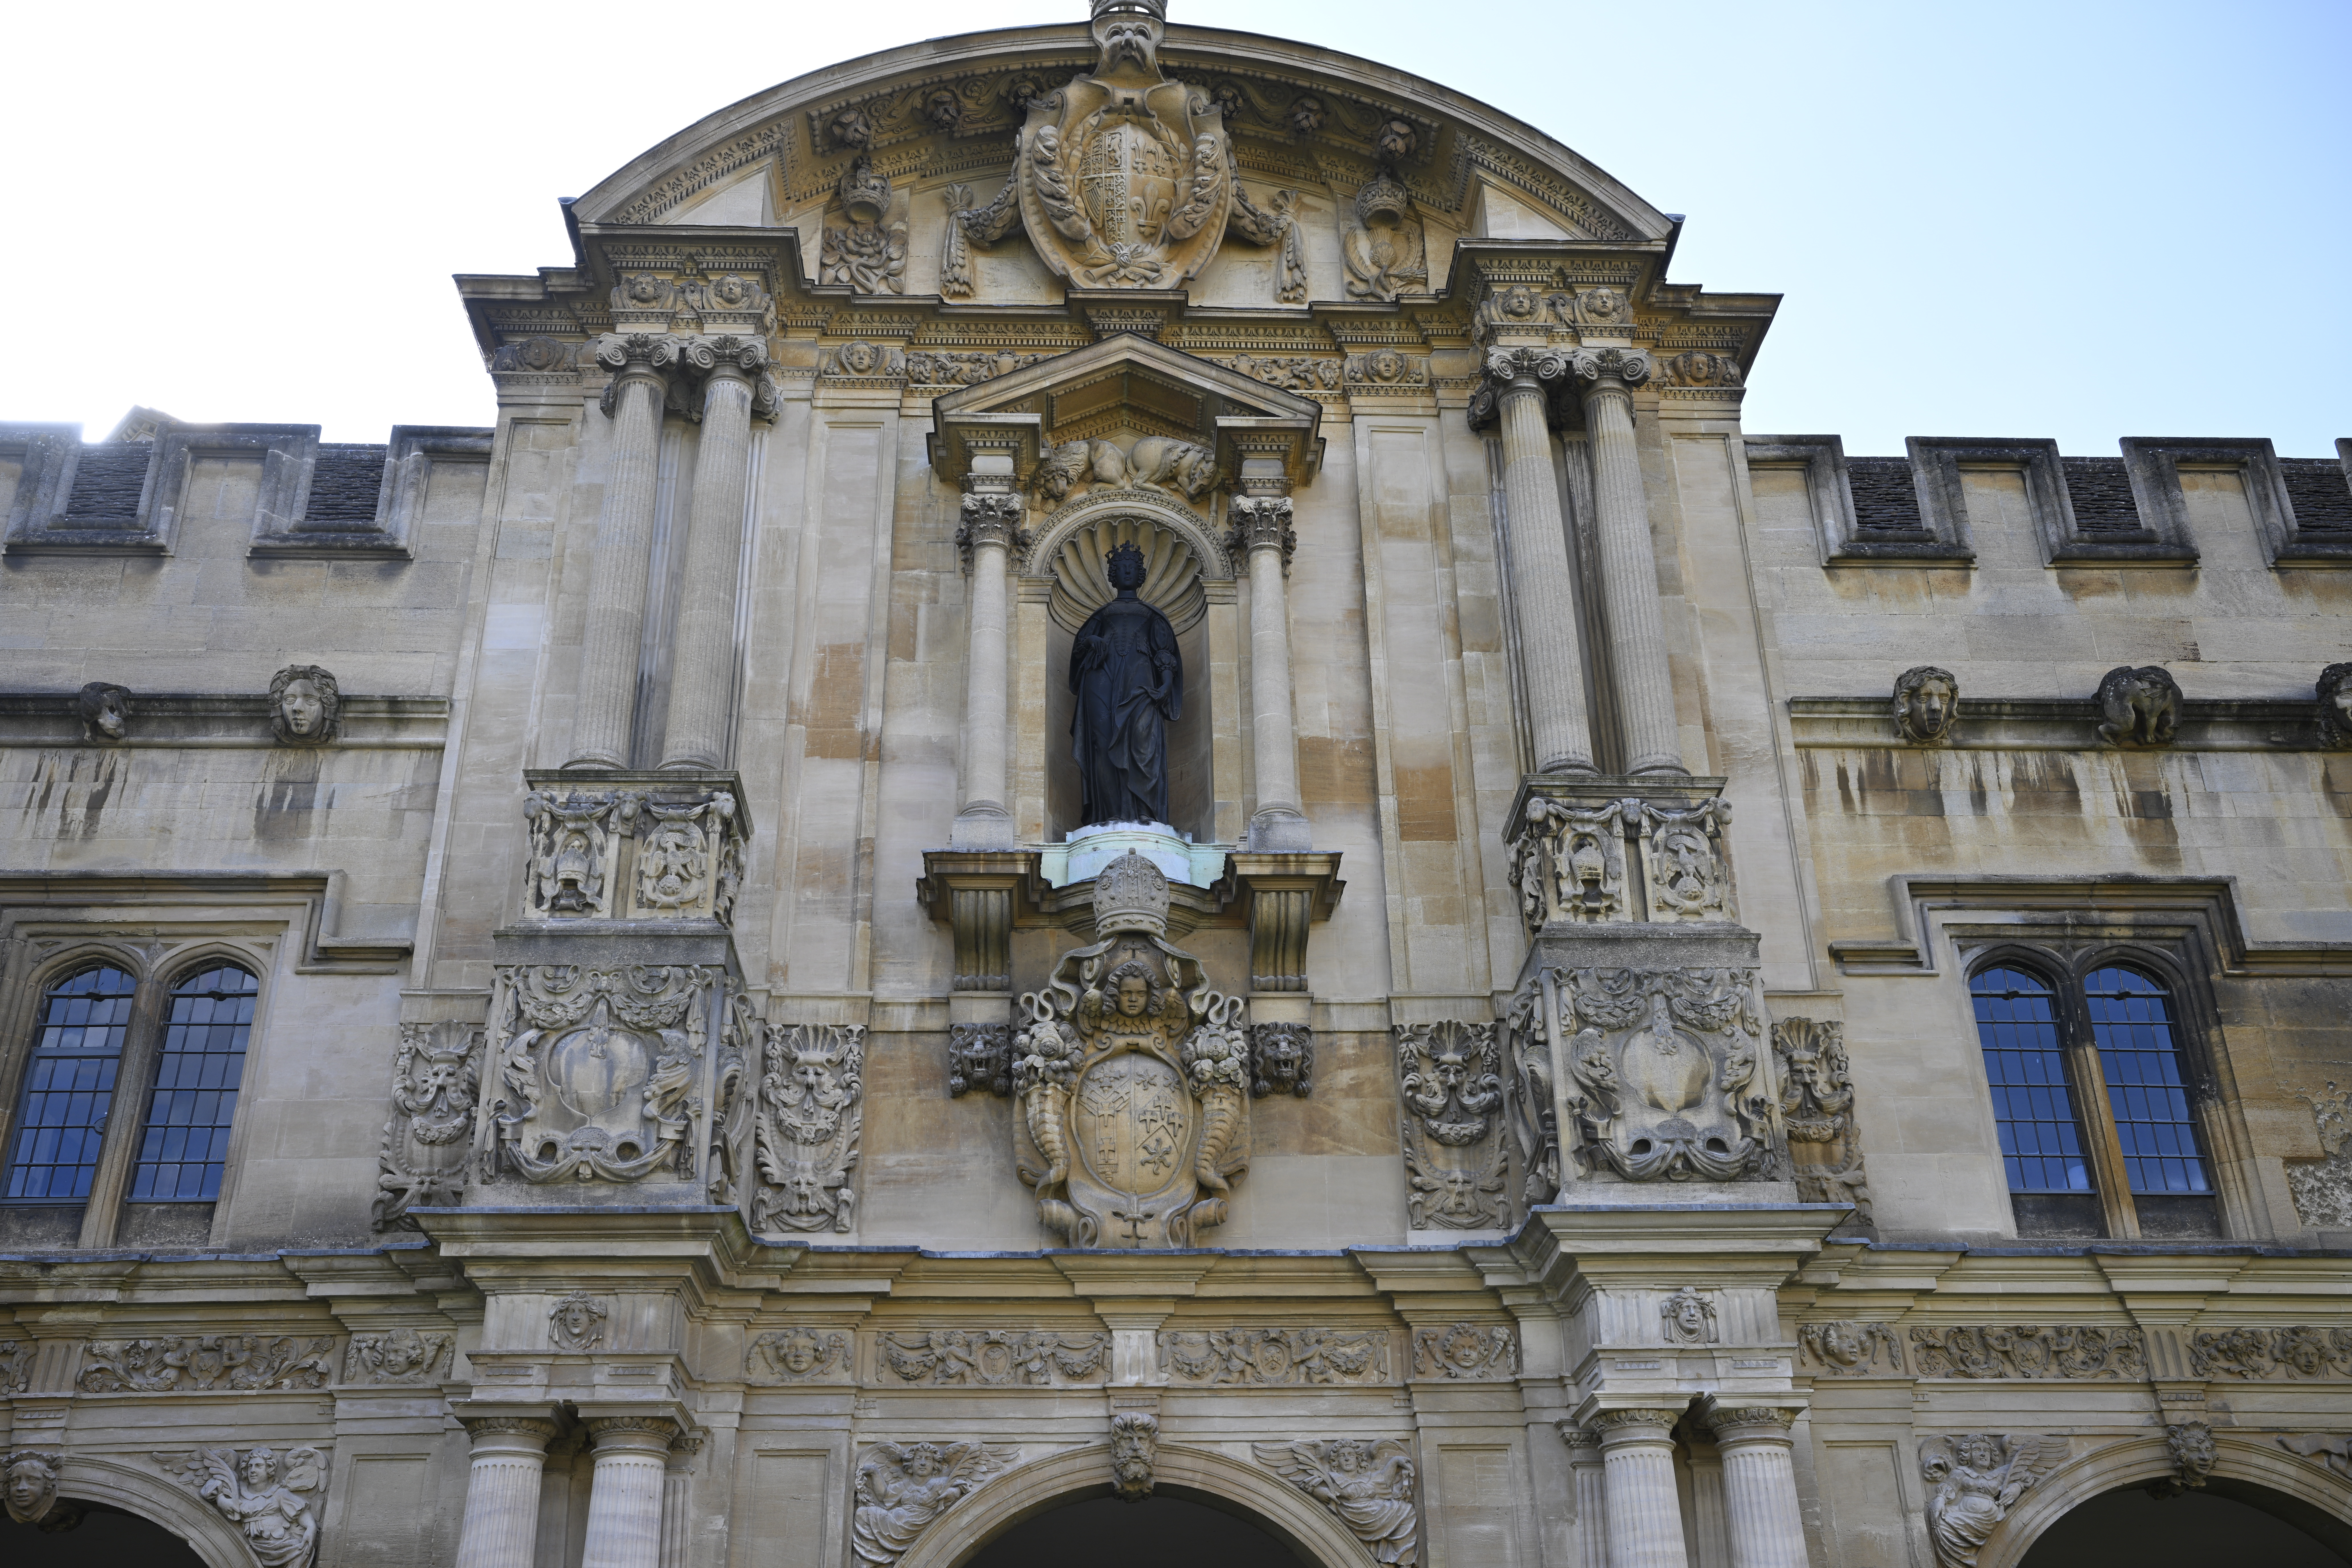
\includegraphics[width=0.24\textwidth, height=0.20\textwidth, keepaspectratio]{figures/Mayowa_Collected/47_clean.jpg} &
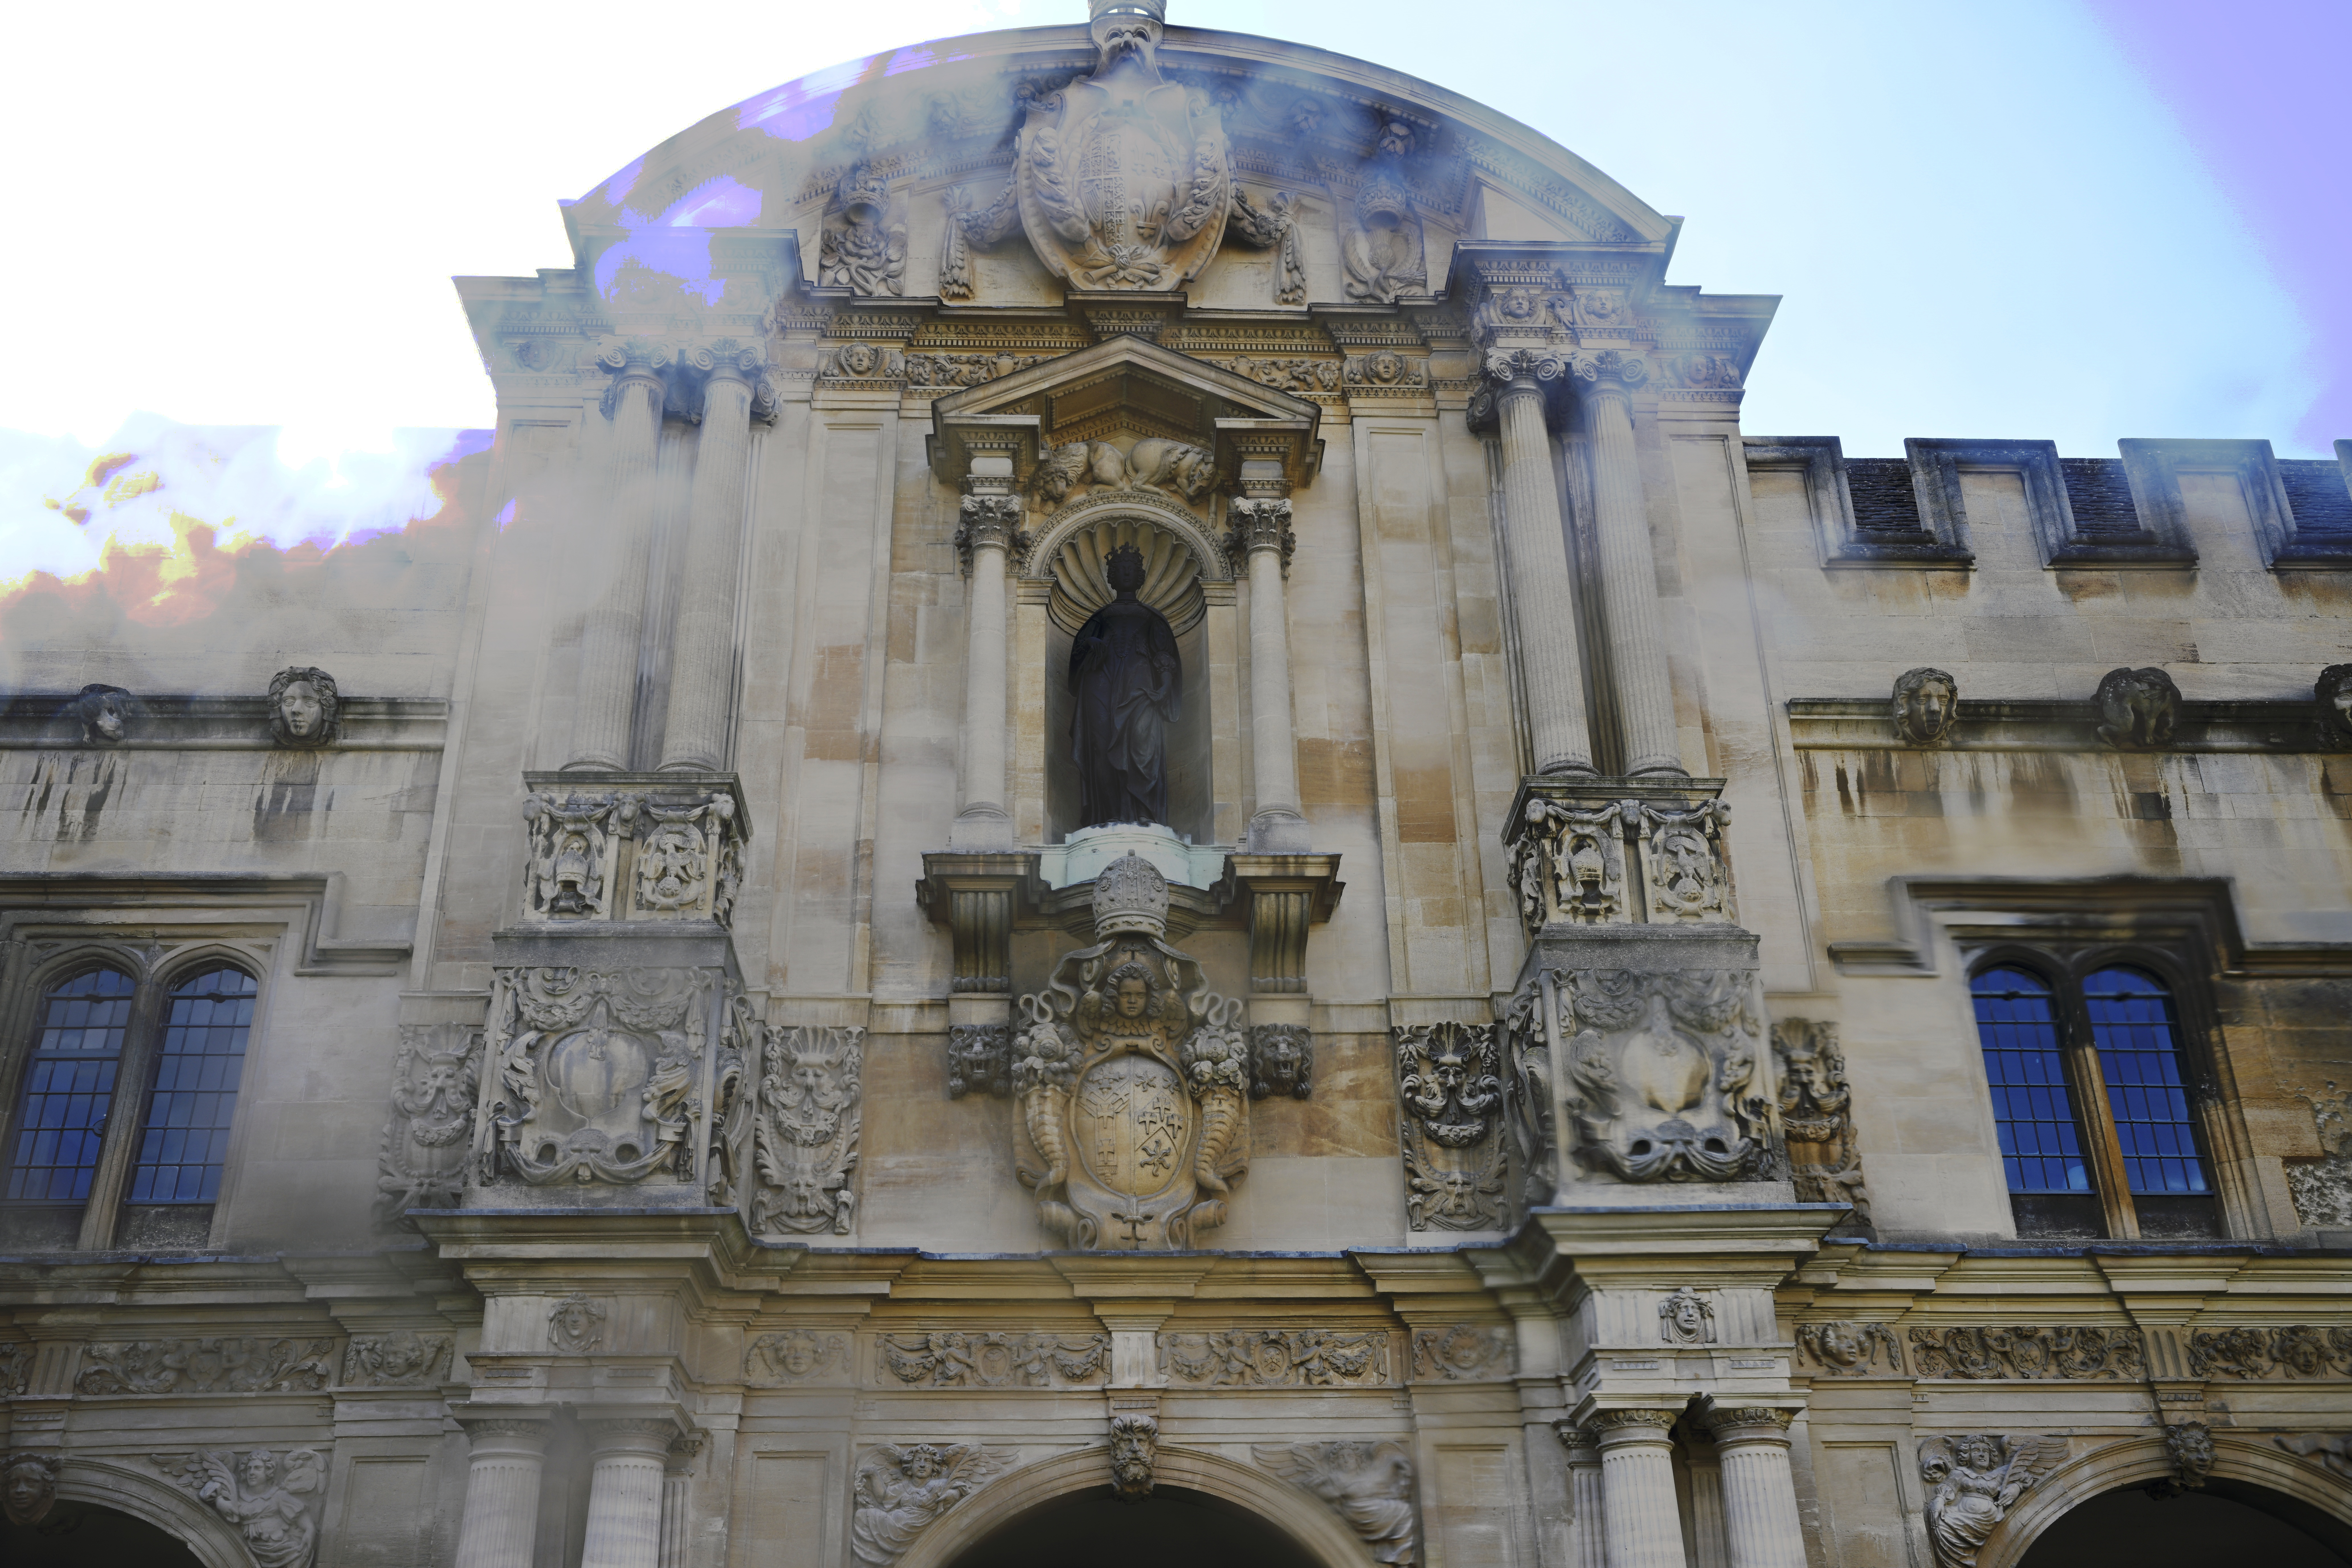
\includegraphics[width=0.24\textwidth, height=0.20\textwidth, keepaspectratio]{figures/Mayowa_Collected/47_30cm.jpg} &
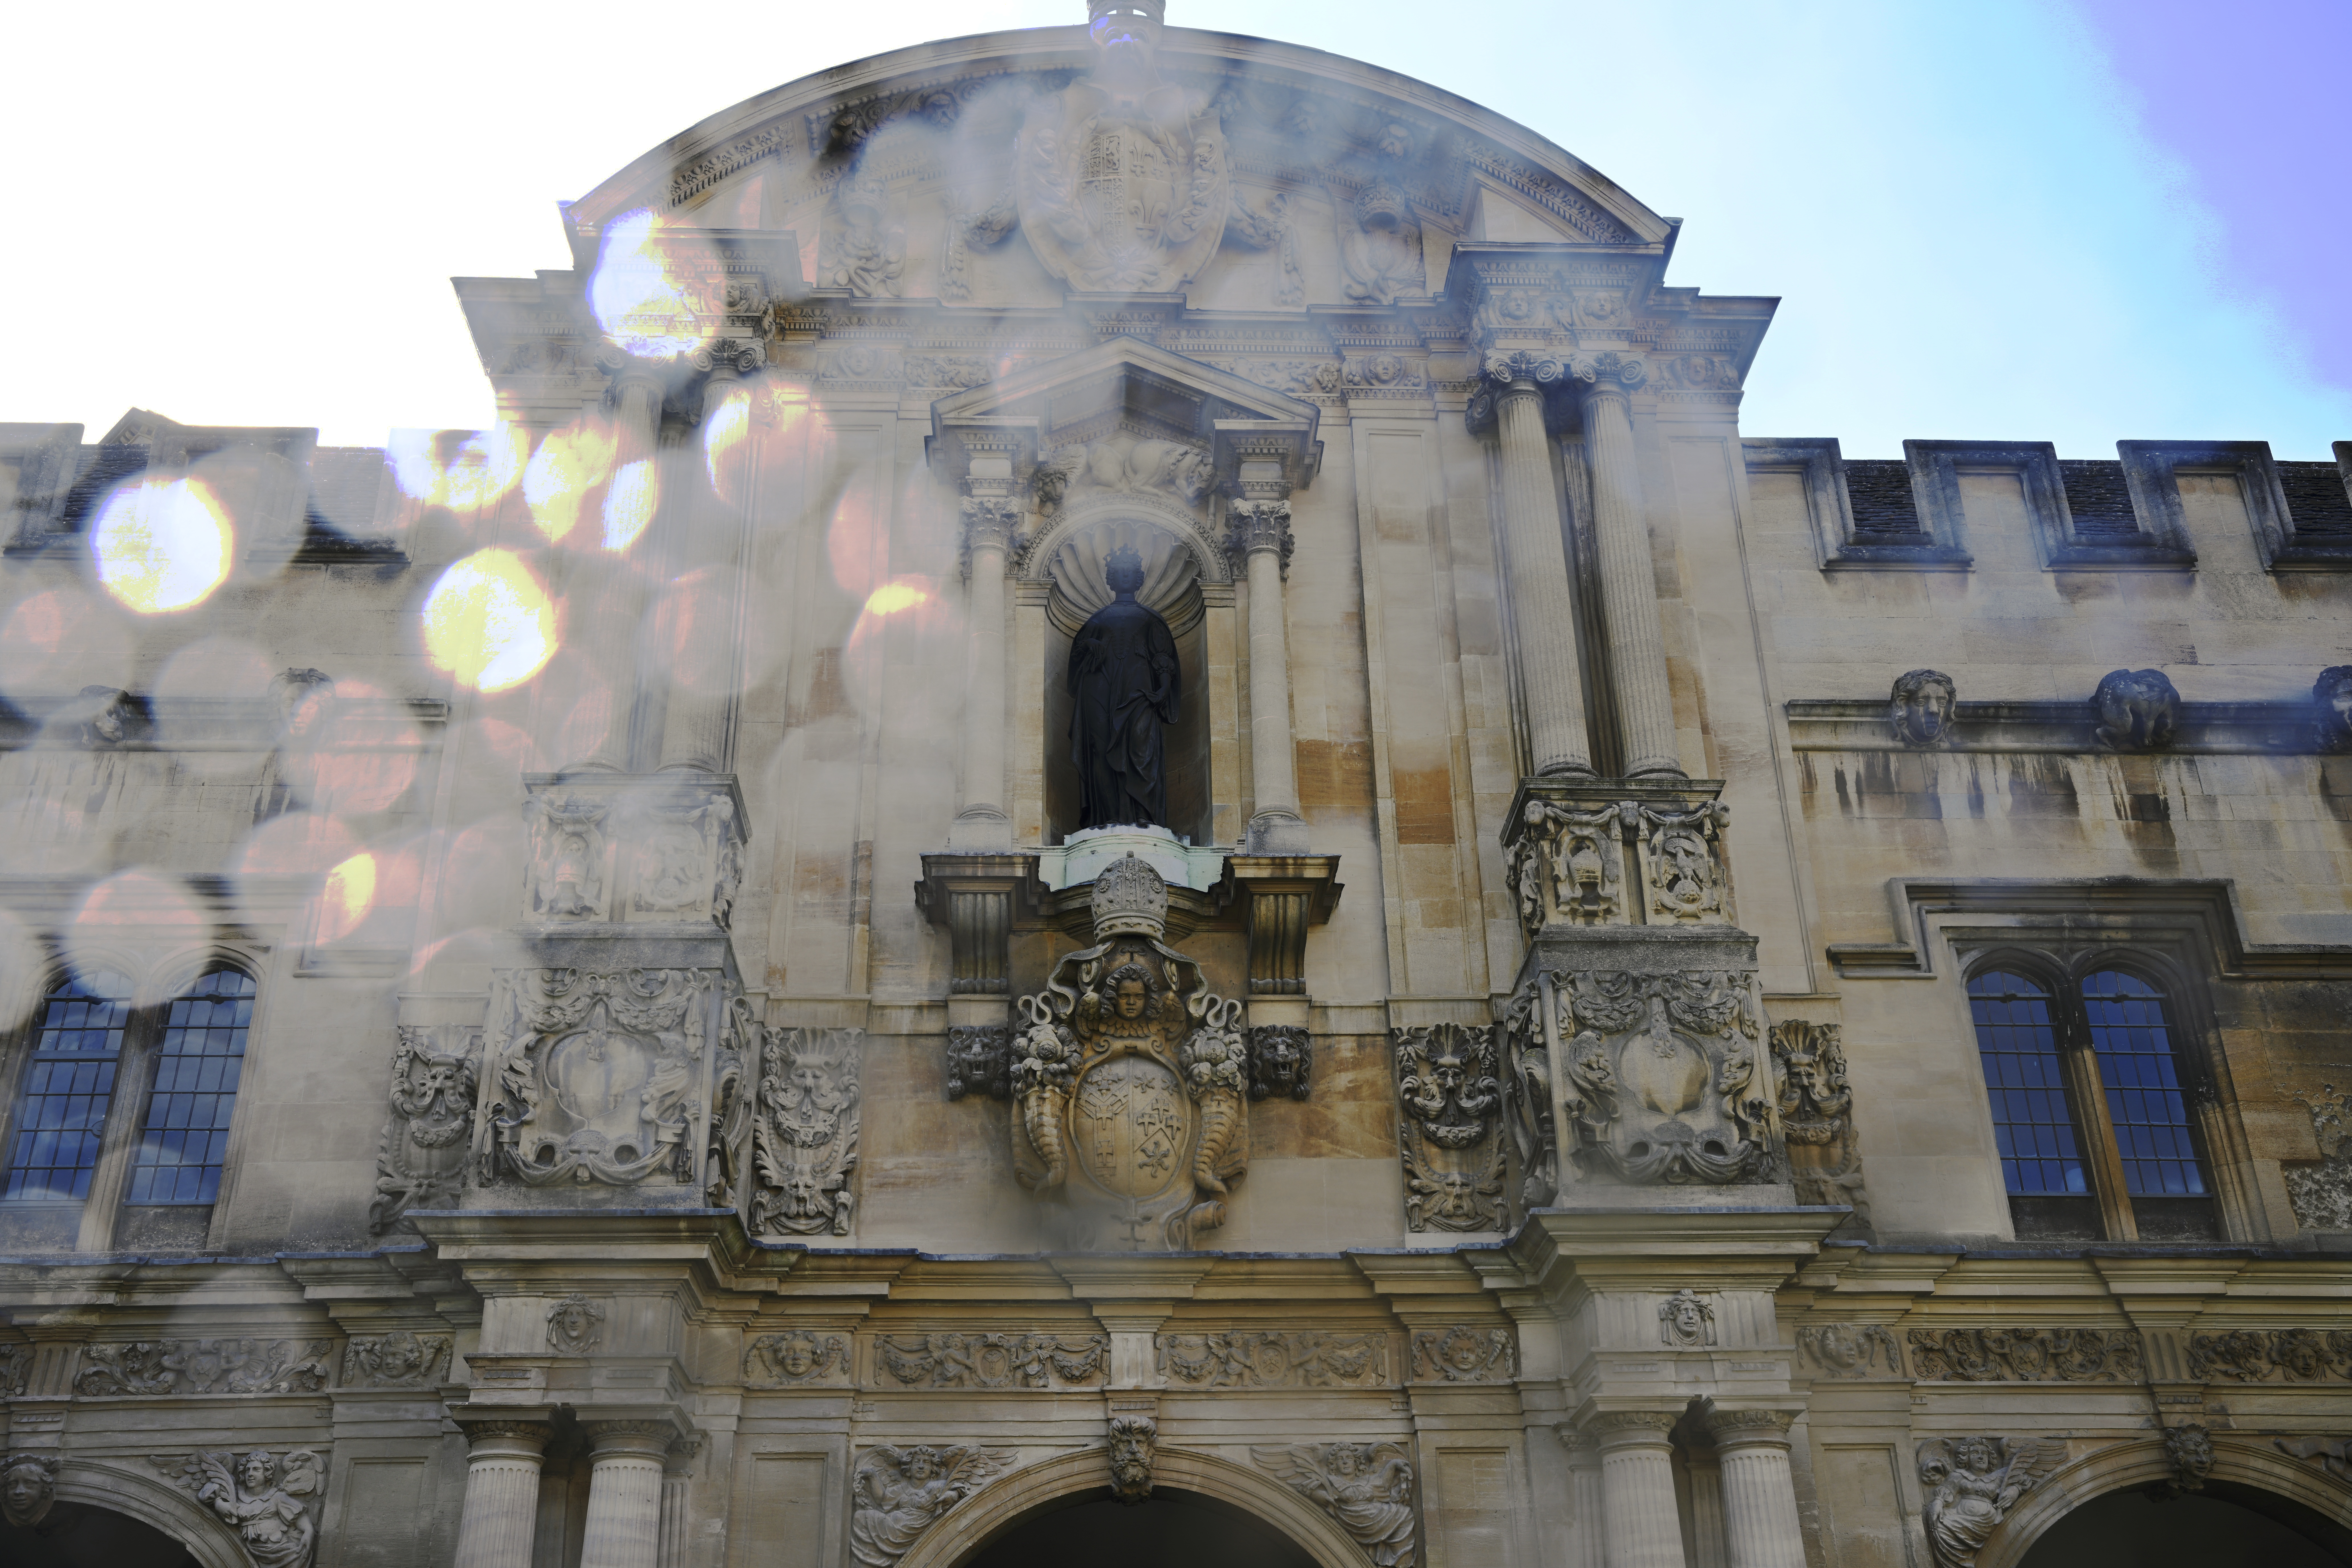
\includegraphics[width=0.24\textwidth, height=0.20\textwidth, keepaspectratio]{figures/Mayowa_Collected/47_50cm.jpg} &
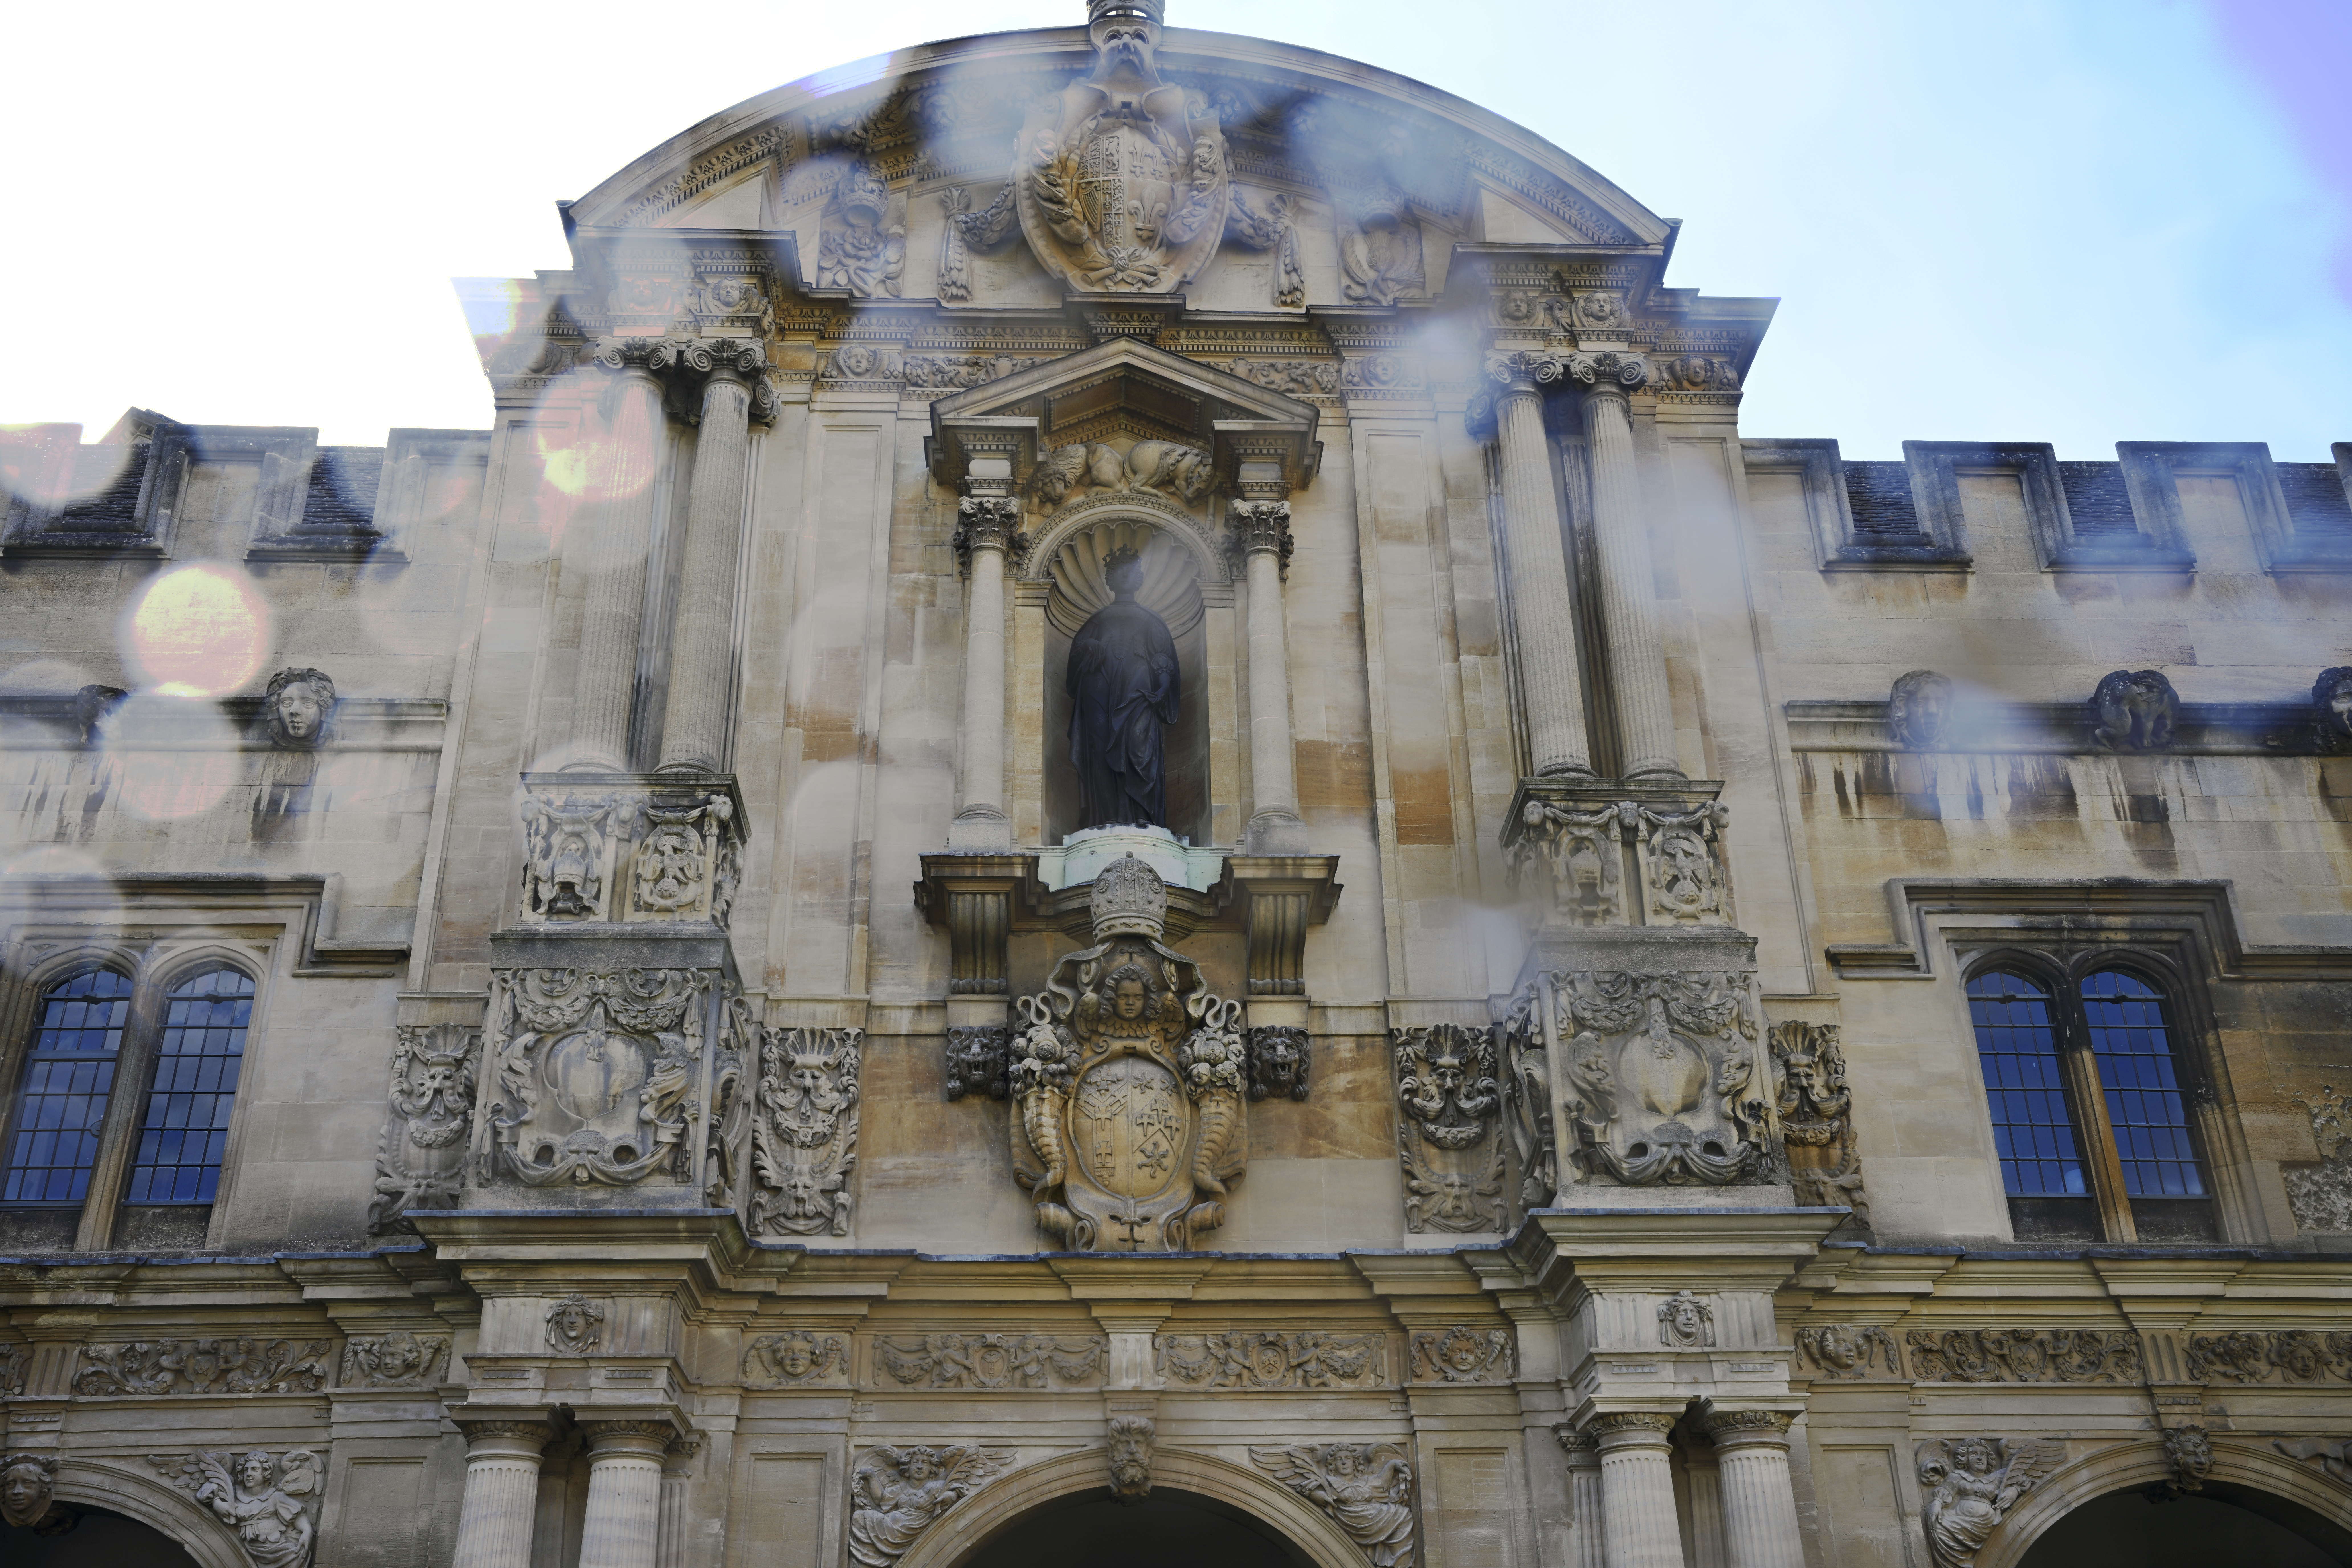
\includegraphics[width=0.24\textwidth, height=0.20\textwidth, keepaspectratio]{figures/Mayowa_Collected/47_70cm.jpg} \\
\end{tabular}
\caption{Example of images captured using data collection protocol detailed}
\label{fig:clean_vs_rain}
\end{figure}


Some processing steps were required before the dataset could be added to the ORDS to enhance the quality and integrity of the images. The day that the images were taken was a very sunny one with no precipitation. One issue that arose during the data collection was the stark difference between the lighting conditions as images for certain backgrounds were taken, this was due to the movement of clouds on the day of collection. So in order to mitigate the different lighting in the images, I decided to apply histogram matching\cite{scikit-image}, which is developed from the concept of histogram equalisation\cite{1975ieht.rept.....H} to all the images. Histogram equalisation is an image processing technique that enhances contrast by redistributing intensity values of the image, aiming for a uniform distribution and making details more visible. The function used in python is a sci-kit image function ,\texttt{skimage.exposure.match\_histogram}, which aligns the histogram of the input image to that of a reference image. For each background (set of four pictures), I chose the initial image captured (the clean image) as the reference image. This approach not only helps in minimizing the lighting inconsistencies but also ensures that the key features are preserved across the dataset.

Further to this, due to the very high resolution of the images captured, a careful downsampling process was necessary to improve computational efficiency while preserving essential visual details. This was implemented using the OpenCV\cite{opencv_library} library’s \texttt{cv2.resize} function with the \texttt{$INTER\textunderscore AREA$} interpolation method, which is particularly well-suited for downsampling, as it helps to avoid aliasing and maintain image quality. Unlike bilinear or bicubic interpolation, which estimate new pixel values based on a small number of neighboring pixels (e.g., bilinear uses only four), \texttt{$INTER\textunderscore AREA$} computes the output by averaging all input pixels that contribute to the area of a single output pixel. This approach reduces high-frequency noise and preserves the overall structure of the image, making it especially effective for tasks involving visual analysis or machine learning inputs\cite{opencv_library}. The images were downsized to $1920 \times 1280$ (width × height) and were then ready for integration into the ORDS. The data collected will be used in this project as a new test set, namely test set D, to evaluate the performance of the models used and developed.

\subsection{Discussion}

The data collection protocol detailed above was successful in collecting a diverse range of data at different locations. As with any method, there were certain limitations. The main issue we faced on the day of data collection were the sharp changes in lighting conditions, due to a high density of cloud cover. These fluctuations contributed to inconsistent illumination, which likely affected the quality of the captured images. I attempted to mitigate the effects of this through histogram matching as detailed in section \ref{section: Data processing}. In future studies, collecting the data on less sunny days can improve the consistency of lighting conditions.

Another limitation in collecting the images was due to the nature of the water sprayer used. The sprayer was very powerful and generated a fast stream of water, which led sometimes to the raindrops smearing onto the glass slabs, instead of landing and remaining in distinct droplets. This issue was further exacerbated due to the human error when spraying onto the glass slab. In order to maintain consistency when collecting data, a constant amount of force should be applied to the sprayer. This was difficult due to the power of the water sprayer, and the inclusion of human error, so some of the spraying distances are not consistent with how they should look.

A method similar to the one used by Porav et al. \cite{8793486} has the potential to mitigate these challenges and help in the procurement of a varied dataset to be used in the extension of the existing dataset. The setup allows one lens of two cameras to be affected by real water droplets while keeping the other lens clear. It contains a 3D printed bi-partite chamber between two clear panels and placed in front of the two lenses, with one side being kept dry and the other sprayed with water droplets using an internal nozzle fitted at the top of the chamber. The paper focuses on the field of view of a vehicle to collect their data. The angle of the chamber with respect to the axes of the cameras can also be changed to simulate a slanted windscreen or a window allowing for more data variability. The nozzle in the chamber is also capable of producing varying diameters of water droplets. There are some potential drawbacks with this method of data collection, one being the complexity of the equipment set up to begin. Something to also consider is that the raindrops will be on the inside of the screen and not the outside like other datasets. However, exploring a dual system such as this can be useful for future studies for fast and consistent collection of data.

\chapter{Recreation of state-of-the-art model}

\section{Introduction}

This chapter describes the state-of-the-art model developed by \cite{Kwon} and my approach to implementing it. I use a proven training strategy that is widely applied in deep learning. I then evaluate the model’s performance on the previously described test sets, both quantitatively and qualitatively. My novel contributions include the full recreation of the model, with the introduction of an additional loss function in training part of the model. Finally, I discuss the model’s limitations and propose potential ways to enhance its performance in future iterations.

\section{Model architecture}
The model proposed by Kwon et al.\cite{Kwon}, shown in figure \ref{fig:Kwon Overall Architecture}, consists of a raindrop‐mask network that identifies raindrop regions, and a raindrop‐removal network that removes the raindrops and recovers a raindrop free image. The raindrop‐mask network is a CNN based on the U-Net architecture, designed to learn the location, shape, and brightness of raindrops. The raindrop‐removal network is a GAN model that combines U-Net with attention modules to identify raindrop areas and restore degraded regions. The first attention module in the removal network is the raindrop mask itself, used as an input alongside the raindrop‐degraded image. The second attention module is a Residual Convolution Block Attention Module (RCBAM), a self‐attention mechanism inserted before the max‐pooling layers in U-Net. 

\begin{figure}
    \centering
    \includegraphics[width=0.8\linewidth]{figures/Kwon-et-al.-Overall-Architecture.png}
    \caption{Overall architecture of the proposed state-of-the-art model}
    \label{fig:Kwon Overall Architecture}
\end{figure}

\subsection{Raindrop mask network}
\label{Subsection:Raindrop mask network}
In order to generate raindrop masks, Kwon et al made changes to the U-Net architecture. The input to the network are raindrop degraded images, while the output images are the raindrop masks. Existing methods before this paper used binary masks or absolute difference masks as the attention maps. These are created by taking the difference between the raindrop-free image and the raindrop-degraded image. To create a binary mask, a threshold is applied to the difference between the degraded and clean images, where pixel values above a certain threshold are labelled as part of the raindrop. This method, however, can introduce noise and lead to inaccuracies in the mask generation as the absolute difference can change the intensity level of the raindrop region meaning the mask is unable to capture the different intensities present in a raindrop. This has an adverse effect on the effectiveness of the raindrop removal. To address this issue, the proposed mask by Kwon et al. is biased to display the negative intensity level. An example is shown in figure \ref{fig:Raindrop masks} where the proposed ground truth mask (d) shows more information about the intensity, shape and size of the raindrop regions better than the absolute difference (c) and binary masks (b), including the dark intensity regions.

\begin{figure}
    \centering
    \includegraphics[width=0.8\linewidth]{figures/Kwon-et-al-Raindrop-Mask-Architecture.png}
    \caption{Raindrop mask architecture. The dimensions shown are the dimensions of the output after the layer.}
    \label{fig:Raindrop mask architecture}
\end{figure}

\begin{figure}
    \centering
    \includegraphics[width=0.5\linewidth]{figures/Kwon-et-al-Raindrop-Masks.png}
    \caption{(a) Raindrop image, (b) binary mask with threshold level 30, (c) absolute difference image, (d) proposed raindrop mask.}
    \label{fig:Raindrop masks}
\end{figure}

Kwon's raindrop masks are generated using equations \ref{Eq:NTSC Formula} and \ref{Eq:Mask Subraction} where the function $f(\cdot)$ transforms a colour image $I$ into a grayscale image and $r$, $g$, and $b$ represent the red, green, and blue channels of the colour image, respectively. $I_{de}$ and $I_{fr}$ represent the raindrop-degraded image and the raindrop-free image, respectively, and $M$ represents the raindrop mask. This mask can then be used to train the raindrop detection.
\noindent
\begin{equation}
f(I) = 0.299 \times r +0.587 \times g+0.114 \times b, 
\label{Eq:NTSC Formula}
\end{equation}
\noindent
\begin{equation} 
M = f(I_{de})-f(I_{fr}),
\label{Eq:Mask Subraction}
\end{equation}
\noindent
The input images to the network are colour images of size $256 \times 256$, with three channels (red, green, blue), and the output raindrop masks are a grayscale image with a single channel. The input images are normalised from $[0,255]$ to $[0,1]$. The raindrop-mask architecture shown in figure \ref{fig:Raindrop mask architecture} consists of several different components similar to the U-Net architecture. The CBR block consists of a convolution layer, batch normalisation, and then a ReLU activation. The downsampling and upsampling layers use max-pooling and two-dimensional (2D) transposed convolution layers, respectively. The skip connections connect the previous layers to the upsampled layers. The skip connections are used to effectively restore information that may be lost in the hierarchical structure when transferring feature maps from the encoder to the decoder, allowing the network to learn the low-level and high-level features and facilitate the integration of detailed information with abstract representation. The skip-connected layers concatenate the previous layers and upsampled layers channel-wise. The convolution layers are applied without the ReLU activation function. All the convolution layers in the mask network use $3 \times 3$ kernels with a stride of 1 and padding of 1. The max-pooling and transposed convolution layers use a $2 \times 2$ kernel with a stride of 2. In the original paper, the loss function used between the generated masks and true masks, calculated using equation \ref{Eq:NTSC Formula} and \ref{Eq:Mask Subraction}, is the mean square error in equation \ref{Eq:MSE}, where $\mathcal{L}_m$ represents the loss for the mask generation, $M$ is the true mask, and $M'$ is the generated mask.
\noindent
\begin{equation}
    \mathcal{L}_m = \mathbb{E}[(M - M')^2],
    \label{Eq:MSE}
\end{equation}
\noindent
The MSE loss is effective at penalizing overall intensity differences but does not necessarily capture the structure and boundaries of raindrops. For example, if the network’s generated mask has slightly mismatched or missing pixels in especially light or dark regions, the MSE may not penalize those differences strongly enough. This occurs around the raindrop edges, leading to incomplete or blurred features in the predicted mask. As a result, relying solely on MSE can hamper the model’s ability to accurately represent the true shape of the raindrops. Building on the method from the paper, I propose an additional loss function for the raindrop mask, the SSIM\cite{SSIM} (Structural Similarity Index Measure) loss. The structural similarity measure by SSIM includes the luminance, contrast and structure of the images. Incorporating this loss function encourages the network to preserve local contrast and shape details in the predicted mask, helping the network highlight the exact raindrop contours better. This enhancement should improve overall performance in the network, as the raindrop masks act as an attention mechanism within the generator. The added clarity of the raindrop contours will help the network more effectively generate a rain-free image. The SSIM loss is defined as:
\noindent
\begin{equation}
\mathcal{L}_{\text{ssim}} = \mathbb{E}\!\Bigg[
  1 - \Biggl(
    \frac{\bigl(2\,\mu_{I_M}\,\mu_{I_{M'}} + \gamma_1\bigr)\,\bigl(2\,\sigma_{I_M\,I_{M'}} + \gamma_2\bigr)}
         {\bigl(\mu_{I_M}^2 + \mu_{I_{M'}}^2 + \gamma_1\bigr)\,\bigl(\sigma_{I_M}^2 + \sigma_{I_{M'}}^2 + \gamma_2\bigr)}
  \Biggr)
\Bigg],
\label{Eq:SSIM}
\end{equation}
\noindent where the right side of the minus term represents the SSIM; $\mu_{I_M}$ \noindent and $\mu_{I_{M'}}$ denote the mean of the true and predicted masks, respectively, while $\sigma_{I_M}^2$ and $\sigma_{I_{M'}}^2$ represent the variance of the masks; \noindent $\sigma_{I_M\,I_{M'}}$ indicates the covariance between the true and predicted masks, and $\gamma_1$ and $\gamma_2$ are constant values of $0.01^2$ and $0.03^2$, respectively. Where $\gamma_1$ and $\gamma_2$ are defined as $(k_1L)^2$ and $(k_2L)^2$, where $L$ is the dynamic range of pixels values which is set equal to $1$ in this paper. As SSIM computes the similarity between two images, the minus term is introduced to utilise it as a loss function. The combination of MSE and SSIM losses should offer a balance between the accuracy of the pixels in the generated mask compared to the true mask, and the structural accuracy. The total mask loss in my training is therefore the addition of the MSE and SSIM losses.

\subsection{Raindrop removal network}

The raindrop removal network is based on a GAN architecture, which consists of a generator and a discriminator. The generator follows the U-Net architecture and incorporates the self-attention module. The discriminator adopts the PatchGAN\cite{PatchGAN} architecture used in Pix2Pix\cite{isola2017image}. The proposed adversarial loss according to the GAN is expressed as:
\noindent
\begin{equation}
\min_{G} \max_{D} \; V(D, G) 
= \mathbb{E}_{I_{fr}}\!\bigl[\log D(I_{fr})\bigr] 
\;+\; \mathbb{E}_{I_{de}}\!\Bigl[\log\bigl(1 - D\bigl(G(I_{de}, M')_1\bigr)\bigr)\Bigr],
\end{equation}
\noindent where $D$ and $G$ \noindent represent the discriminator and generator, respectively. Here, \( I_{fr} \) denotes the raindrop-free image, and \( I_{de} \) represents the raindrop-degraded image and $M'$ represents the generated mask as before. As seen in the equation, $G(\cdot)$ represents the generator generating a rain-free image from the input rain degraded image and generated mask, with the $1$ subscript denoting the first output. $D(\cdot)$ then represents the discriminator assessing the authenticity of an image, classifying it as real or fake. The first term in the equation is the discriminator classifying the true rain-free image and therefore the discriminator aims to maximise this term. The discriminator also aims to maximise the second term by correctly classifying the images generated by the generator as fake. The generator aims to minimise this term to fool the discriminator to incorrectly classify the generated images as real. This ensues a zero sum game between the generator and the discriminator where the generator attempts to minimise the loss function and the discriminator attempts to maximise it. The generator improves its generation process based on the feedback from the discriminator while the discriminator enhances its ability to distinguish real images from generated ones.

\subsubsection{Generator}

The generator input is a channel-wise concatenation of the raindrop-degraded image and the generated mask leading to input dimensions of $256 \times 256 \times 4$. The output image is the generated clean image, where the generator produces multiple output images with different resolutions at $256 \times 256$, $128 \times 128$, and $64 \times 64$. The generator architecture comprises of the same layers as in the raindrop-mask network, with the addition of the self-attention RCBAM layer. The CBR layers are also replaced with CBL ones that comprises a convolution, batch-normalisation and leakyReLU activation function applied. The architecture is shown in figure \ref{fig:Generator architeture}. All convolution layers in the generator use $3 \times 3$ kernels with a stride of $1$ and padding of $1$, and the max-pooling and transposed convolution layers use $2 \times 2$ kernels with a stride of 2. The negative slope of the LeakyReLU is $0.2$.

\begin{figure}
    \centering
    \includegraphics[width=0.9\linewidth]{figures/Kwon-et-al-Generator-Architecture.png}
    \caption{Generator architecture. Dimensions shown are the dimensions of the output after the layer.}
    \label{fig:Generator architeture}
\end{figure}

RCBAM, based on the Convolution Block Attention Module (CBAM)\cite{woo2018cbam}, is used to improve the model performance by effectively restoring the raindrop area with the input raindrop mask. The CBAM comprises channel and spatial-attention modules. The channel-attention module is used to find areas with important meaning in the image, while the spatial-attention module is used to find the position of a meaningful region in the image. The equations governing the CBAM are as follows:
\noindent
\begin{equation}
CA(I) = \sigma \bigl(
   \mathrm{MLP}(\mathrm{AvgPool}(I))
   \;+\;
   \mathrm{MLP}(\mathrm{MaxPool}(I))
\bigr),
\end{equation}
\noindent
\begin{equation}
SA(I) = \sigma \Bigl(
   \mathrm{conv}_{7\times7}\bigl(
     Concat(AvgPool(I),MaxPool(I)
   \bigr)
\Bigr),
\end{equation}
\noindent where $CA(\cdot)$ and \noindent $SA(\cdot)$ denote the channel-attention and spatial-attention outputs, respectively; $\sigma(\cdot)$ refers to the sigmoid activation function; $\mathrm{MLP}$ denotes a multi-layer perceptron with a convolution of kernel size $1 \times 1$, a ReLU activation function and another convolution of the same size kernel; and $\mathrm{conv}_{7 \times 7}$ represents a convolution with kernel size $7 \times 7$. The structure of the RCBAM used is in figure \ref{fig:RCBAM architeture}, where the residual block using a skip connection with a convolution of $3 \times 3$ kernel size is what differs it from the CBAM.

\begin{figure}
    \centering
    \includegraphics[width=0.5\linewidth]{figures/Kwon-et-al-RCBAM.png}
    \caption{RCBAM structure.}
    \label{fig:RCBAM architeture}
\end{figure}

The generator uses four loss functions: adversarial loss, perceptual loss, SSIM loss, and multiscale MSE loss. The adversarial loss is expressed in equation \ref{Eq:Adversarial loss}, where \( G(I_{de}, M')_1 \) denotes the first output of the generator \( G \) given the rain-degraded input \( I_{de} \), also denoted as $I_{ge1}$, and the model generated mask \( M' \). 
\noindent
\begin{equation}
\mathcal{L}_{\text{adv}}
= \mathbb{E}\!\Bigl[\log \bigl(1 - G(I_{de}, M')_1\bigr)\Bigr],
\label{Eq:Adversarial loss}
\end{equation}
 
The perceptual loss aims to measure the perceptual similarity of the two images by generating feature maps of the target image and the generated output using pretrained networks. The pretrained network has been trained to detect edges, textures and patterns and contain this information in the feature maps. The pretrained network used is VGG19\cite{simonyan2014vgg}. The equation is then used extract the difference between these feature maps and guides the model to minimise this. The perceptual loss is defined in equation \ref{Eq:Perceptual loss} where $\phi(\cdot)$ represents the feature map of the pre-trained VGG19 network and all other terms are as defined previously.
\noindent
\begin{equation}
\mathcal{L}_{\text{per}} = \mathbb{E}\!\Bigl[\bigl(\phi(I_{fr}) - \phi(I_{ge1})\bigr)^2\Bigr].
\label{Eq:Perceptual loss}
\end{equation}

The SSIM loss is the same as defined in the raindrop mask generator in section \ref{Section:Raindrop mask network}, with the true mask and generated mask images replaced with the ground truth raindrop-free image and the first generated raindrop-free image. The $\gamma_i$ values are the same as originally set in the paper.

The multiscale MSE loss\cite{qian2018attentive} is a method for calculating loss by extracting features from different layers of the decoder in the generator, here from the 3 outputs of the generator. Each extracted feature map corresponds to a different scale. Considering multiple scales, multiscale losses can capture more contextual information from different scales. The multiscale loss is expressed in equation \ref{Eq:Multiscale loss}, where $S(\cdot)_i$ represents a resizing function to match the true rain-free image to the output $i$ of interest. The total loss is the sum of all these loss functions.
\noindent
\begin{equation}
\mathcal{L}_{\text{mul}} = \frac{1}{3}\sum_{i=1}^{3} \mathbb{E}\!\Bigl[\bigl(S(I_{fr})_i - I_{{ge}{_i}}\bigr)^2\Bigr].
\label{Eq:Multiscale loss}
\end{equation}

\subsubsection{Discriminator}

The discriminator is used with the aim of improving the performance of the generator by effectively distinguishing between the generated images and the ground truth. The discriminator based on PatchGAN considers local $N \times N$ patches where $N$ is equal to $70$. Unlike PixelGAN which considers whether the input images are real/fake by considering each pixel independently. This discriminator uses a texture style loss allowing it to generate more high-frequency components by treating each patch independently. The size of $N$ chosen results in higher sharpness in both spatial and colour dimensions\cite{isola2017image}. The sharpness here represents the reproduction of high frequency content in the image, which include clear edges and textures (spatial sharpness), and also vivid, unsmudged colours (colour sharpness). The discriminator used in the proposed model is shown in figure \ref{fig:Discriminator architeture}. The first CL block comprises a convolution layer and the LeakyReLU activation function. The CBL layer is as defined previously. The CS layer comprises a convolution layer and the sigmoid activation function. All the convolution layers in the discriminator use a $4 \times 4$ kernel size with a stride of $2$ and a padding of $1$. The negative slope of the LeakyReLU function is set to $0.2$.
\begin{figure}
    \centering
    \includegraphics[width=0.3\linewidth]{figures/Kwon-et-al-Discriminator-Architecture.png}
    \caption{Discriminator architecture}
    \label{fig:Discriminator architeture}
\end{figure}
The loss of the discriminator is expressed in equation \ref{Eq:Discriminator loss} with all terms as previously defined.

\begin{equation}
\mathcal{L}_D = \mathbb{E}\!\Bigl[\log D(I_{fr})\Bigr]
+ \mathbb{E}\!\Bigl[\log\Bigl(1 - D\bigl(I_{ge_{1}}\bigr)\Bigr)\Bigr].
\label{Eq:Discriminator loss}
\end{equation}

\section{Training}
In this section I will outline the training strategy I used to train my implementation of the model. I also accessed the original code written by Kwon et al.\cite{Kwon} through the Github repository at https://github.com/Hyukju/Raindrop-Removal.git. Here I will outline my training strategy and the datasets used in my experiment after. 

\subsection{Training strategy}
\label{Section:Training strategy}
In order to ensure that the model is generalisable to to a wide range of data, I choose to employ K-Fold cross validation (CV)\cite{stone1974cross}. This checks if the results are consistent within varying subsets of the dataset. The choice of K has been written about in literature, with the most common values being $K=5$ or $K=10$ as these are values suggested to give test error rates estimates that do not suffer from extremely high bias or variance\cite{marcot2021optimal}\cite{nti2021performance}. Also, a general rule is that the larger the dataset, the lower the value of K should be\cite{Parmeet_Report}. Due to the data augmentation performed on our dataset we are left with a large number of images to train on, almost $18000$. Taking in to account all of this alongside computational complexity, in this instance, I utilized a 5-fold CV approach, where the dataset was partitioned into five distinct subsets. The model was trained on four subsets while the remaining subset served as the validation set, this is repeated five times so all subsets are the validation subset once. The model is also trained end-to-end, meaning the mask generation network and the raindrop removal networks are both trained together inside an end-to-end model. The training strategy is as follows:

\begin{enumerate}
    \item Perform K-Fold CV with $K=5$, saving the weights of the model that performs the best on the validation set during training. Each fold was trained for $50$ epochs. The validation loss is tracked throughout so that if an epoch produces the current lowest validation loss the weights for that fold are saved at that epoch, this process is repeated until training finishes. 
    \item Evaluate the performance of the saved models on their respective validation sets using certain metrics. The summary statistics include:

    For the raindrop mask part of the network, I used the MSE and the SSIM in equations \ref{Eq:MSE} and \ref{Eq:SSIM} respectively. 
    The raindrop removal generator uses the same SSIM equation replacing the true and generated masks, with the raindrop-free image and raindrop-degraded image. I also then use the PSNR\cite{TANCHENKO2014874} as a measure of the quality of the generated images. The PSNR measures the proximity of the corresponding pixels between a generated image and the original image. It is the ratio of the maximum power of a signal to the power of corrupting noise that affects the fidelity of its representation. The PSNR is calculated using the following equation:

    \begin{equation}
        PSNR = 20 \log_{10}\Bigr(\frac{MAX}{MSE(I_{ge_{1}},I_{fr})}\Bigr),
        \label{Eq:PSNR}
    \end{equation}
    where $MAX$ represents the maximum pixel value of the images, and the MSE is as defined before. The higher the PSNR, the better the quality of the image.
    \item Choose the best model by assessing an aggregate of the z-normalised summary statistics.
    To determine which model had the best performance, I first standardise the results of the different folds to bring them to a common scale using z-score normalisation, centering the data around a mean of 0 and standard deviation of 1. The data was normalised using equation \ref{Eq: Standardise} with z being the standardised score, x is the original value, $\mu$ is the mean of the samples and $\sigma$ is the standard deviation of the samples.
    \begin{equation}
        z = \frac{x - \mu}{\sigma}
        \label{Eq: Standardise}
    \end{equation}
    For the mask generator, the total z-score was the SSIM score - MSE score. This is because I want to maximise the SSIM and minimise the MSE so the highest SSIM - MSE score gives the best performing model. For the raindrop removal generator, the total z-score was the PSNR score + SSIM score. This is because I want to maximise both the PSNR and SSIM, so the highest score from adding the two metrics is the best score. Since the model is trained end-to-end, the overall score of each distinct model is the sum of the mask generator z score and the removal generator z score.
    \item Retrain the model with the best z score using the saved weights and for the same number of epochs these weights were saved at, on the entire dataset. 
    \item Save the weights at the end of this training process (i.e, all 5 folds), giving the best performing model.
\end{enumerate}

The proposed method was used to train both my implementation of the network, and by Parmeet et al.\cite{Parmeet_Report} to train their implementation of the network. The original paper does not mention a specific training strategy, except that they train their model for 1800 epochs and saved the resulting weights. I trained the model from the original paper for the same number of epochs as my best model from my training strategy, essentially taking their training strategy to be the training over 1800 epochs. All models were trained on the augmented dataset C from table \ref{table:dataset_c}, and also tested on the same datasets. 

Adam optimisers\cite{kingma2014adam} are used in the models, with the hyperparameters set to $\beta_{1} = 0.5$, $\beta_2 = 0.999$, and a learning rate of $0.0002$, in all three models. The generators and discriminators are also initialised from a Gaussian distribution with a mean of 0 and a standard deviation of 0.02 in all models. The high performance computing cluster I use to train and test the model uses a Tesla V100-PCIE-32GB GPU. 

\section{Results}
This section contains all the results throughout my training and testing. For the training, I will only focus on the results from my implementation for brevity, I will then compare the results for the testing for all the models. There are some differences between the models I am assessing here and I will outline them briefly. Henceforth, I will define 3 models; model 1 will be my implementation of Kwon's model, model 2 will be the retrained model from the original paper\cite{Kwon}, and model 3 will be the implementation by Parmeet et al\cite{Parmeet_Report}. 

\begin{table}[h]
    \centering
    \begin{tabular}{l c c c}
    \hline
         & \textbf{End-to-End} & \textbf{Mask-loss} \\
    \hline
    \textbf{Model 1} & \checkmark  & MSE + SSIM \\
    \textbf{Model 2} & \checkmark  & MSE \\
    \textbf{Model 3} & \times & MSE \\
    \hline
    \end{tabular}
    \caption{Table illustrating differences in the 3 models discussed in section 4}
    \label{tab:Different models}
\end{table}

Models 1 and 2 are designed as end-to-end systems that simultaneously train both the mask generator and the removal generator, as they function within a unified framework. While model 3 separates the two networks and trains the mask generator first using the K-Fold CV detailed above finding the best model, then generating masks from the training data using the trained model. Then the raindrop removal network is trained separately using the mask generator generated masks and the input images. The other difference is the loss used to train the mask generator, I proposed the addition of SSIM loss into the total loss for the mask. Apart from these differences, everything else in the models is the same as they all follow the same architecture.


\subsection{Quantitative results}
I will begin this section by discussing the quantitative results achieved by the best models in each fold in my training strategy. These results are shown in figures \ref{tab:Mask generator fold results} and \ref{tab:Removal generator fold results}.
\begin{table}[ht]
\centering
\begin{tabular}{|l|c|c|c|c|c|}
\hline
 & Fold 0 & Fold 1 & Fold 2 & Fold 3 & Fold 4 \\
\hline
\makecell{Mean MSE $\pm$ \\ STD} & 
\makecell{0.006784 $\pm$ \\ 0.004220} & 
\makecell{0.01314 $\pm$ \\ 0.01596} & 
\makecell{0.005581 $\pm$ \\ 0.002643} & 
\makecell{0.006297 $\pm$ \\ 0.004605} & 
\makecell{0.005188 $\pm$ \\ 0.002191} \\
\hline
\makecell{Mean SSIM $\pm$ \\ STD} & 
\makecell{0.7617 $\pm$ \\ 0.1231} & 
\makecell{0.8499 $\pm$ \\ 0.07453} & 
\makecell{0.8101 $\pm$ \\ 0.09001} & 
\makecell{0.8211 $\pm$ \\ 0.08735} & 
\makecell{0.8173 $\pm$ \\ 0.08342} \\
\hline
Epoch Saved & 39 & 44 & 4 & 6 & 5 \\
\hline
\end{tabular}
\caption{Best performing models for each fold in mask generator K-Fold training strategy.}
\label{tab:Mask generator fold results}
\end{table}

\begin{table}[ht]
\centering
\begin{tabular}{|l|c|c|c|c|c|}
\hline
 & Fold 0 & Fold 1 & Fold 2 & Fold 3 & Fold 4 \\
\hline
\makecell{Mean PSNR $\pm$ \\ STD} & 
\makecell{22.7655 $\pm$ \\ 2.5104} & 
\makecell{25.4398 $\pm$ \\ 1.7394} & 
\makecell{23.5932 $\pm$ \\ 1.5377} & 
\makecell{24.3348 $\pm$ \\ 1.5142} & 
\makecell{23.4113 $\pm$ \\ 1.2146} \\
\hline
\makecell{Mean SSIM $\pm$ \\ STD} & 
\makecell{0.8032 $\pm$ \\ 0.08502} & 
\makecell{0.8649 $\pm$ \\ 0.03918} & 
\makecell{0.8394 $\pm$ \\ 0.04219} & 
\makecell{0.8468 $\pm$ \\ 0.03753} & 
\makecell{0.8382 $\pm$ \\ 0.03835} \\
\hline
Epoch Saved & 39 & 44 & 4 & 6 & 5 \\
\hline
\end{tabular}
\caption{Best performing models for each fold in raindrop removal generator K-Fold training strategy.}
\label{tab:Removal generator fold results}
\end{table}
For these results, the averages across all folds are as follows, for the raindrop mask network the average MSE and SSIM are, MSE:$0.0074 \pm 0.0029$, SSIM:$0.8129\pm 0.0286$. This shows the model to be generalisable to varying subsets of data as the variation in these results remain relatively low, similar to the variation in each individual fold. For the raindrop removal generator, the average PSNR and SSIM are; PSNR:$23.9089\pm 0.9143$, SSIM:$0.8385\pm 0.0200$, where again we see low variability across all the folds, showing the model is generalisable. As my implementation is a unified framework much like the original, I will consider the z-scores of each fold's mask generator and removal generator together. The scores after using the standardisation formula is shown in table \ref{tab:Z-scores for my model}. The bold figure in the final row depicts the best performing fold through this method which is fold 1. In this instance, I retrained the model using the saved weights for fold 1, training for 44 epochs. I also train model 2, the model from the original paper for the same number of epochs. 

\renewcommand{\arraystretch}{1.3}    % row spacing
\setlength{\tabcolsep}{10pt}        % column spacing

\begin{table}[ht]
\centering
\begin{tabular}{|l|c|c|c|c|c|}
\hline
 & Fold 0 & Fold 1 & Fold 2 & Fold 3 & Fold 4 \\
\hline
Mask MSE & -0.2099 & 1.9638 & -0.6212 & -0.3765 & -0.7559 \\
\hline
Mask SSIM & -1.7617 & 1.3251 & -0.0681 & 0.3176 & 0.1870 \\
\hline
SSIM - MSE & -1.5518 & -0.6387 & 0.5534 & 0.6941 & 0.9430 \\
\hline
Generator PSNR & -1.2506 & 1.6744 & -0.3453 & 0.4657 & -0.5442 \\
\hline
Generator SSIM & -1.7591 & 1.3165 & 0.0442 & 0.4124 & -0.0141 \\
\hline
PSNR +  SSIM & -3.0097 & 2.9909 & -0.3011 & 0.8782 & -0.5583 \\
\hline
Total score & -4.5615 & \textbf{2.3523} & 0.2523 & 1.5723 & 0.3847 \\
\hline
\end{tabular}
\caption{Z scores for the raindrop mask network and raindrop removal network in the unified framework}
\label{tab:Z-scores for my model}
\end{table}

I now evaluate the resulting models, Model 1 and Model 2, on the various test sets (A, B, C, and D). Given that the main difference between Model 1 and Model 2 is the addition of SSIM loss to the mask generator loss function, I compute the test results for both the mask generator and the raindrop removal generator for each model. Since I was unable to run the code for Model 3, I only have final results for the raindrop removal generator on test sets A, B, and C. All models are trained on dataset C so they can be fairly evaluated on these test sets to ensure a proper comparison. In the interest of brevity, and because the variation among the datasets is less critical and the different parts of the networks for the same metrics and datasets all show similar standard deviations, I have decided to omit the standard deviation term in the displayed test results. The results shown are still the average of the metrics over the test data. For clarity, the emboldened results in each column will be the best performing for that column, and the second best will be underlined. The results are shown in tables \ref{tab:Mask generator test results} and \ref{tab:Removal generator test results}. The results clearly show the recreation of the state-of-the-art model was a success.

\begin{table}[ht]
\centering
\begin{tabular}{|c|cc|cc|cc|cc|}
\hline
\multirow{2}{*}{} 
  & \multicolumn{2}{c|}{Test Set A} 
  & \multicolumn{2}{c|}{Test Set B} 
  & \multicolumn{2}{c|}{Test Set C} 
  & \multicolumn{2}{c|}{Test Set D} \\
\cline{2-9}
 & MSE\downarrow & SSIM\uparrow & MSE\downarrow &  SSIM\uparrow  & MSE\downarrow &  SSIM\uparrow  & MSE\downarrow &  SSIM\uparrow  \\
\hline
Model 1 & 0.1469 & \textbf{0.7701} & \textbf{0.0053} & \textbf{0.6840} & 0.1125 & 0.7199 & 0.0867 & 0.5741 \\
\hline
Model 2 & \textbf{0.0156} & 0.7159 & 0.0058 & 0.6478 & \textbf{0.0026} & \textbf{0.7458} & \textbf{0.0041} & \textbf{0.5868} \\
\hline
Model 3 & - & - & - & - & - & - & - & - \\
\hline
\end{tabular}
\caption{Raindrop mask generator results on all test sets for generated masks. For the MSE and SSIM metrics. Up arrows indicate metrics where higher score is better and vice versa for down arrows.}
\label{tab:Mask generator test results}
\end{table}

\begin{table}[ht]
\centering
\begin{tabular}{|c|cc|cc|cc|cc|}
\hline
\multirow{2}{*}{} 
  & \multicolumn{2}{c|}{Test Set A} 
  & \multicolumn{2}{c|}{Test Set B} 
  & \multicolumn{2}{c|}{Test Set C} 
  & \multicolumn{2}{c|}{Test Set D} \\
\cline{2-9}
 & PSNR\uparrow &  SSIM\uparrow  & PSNR\uparrow &  SSIM\uparrow  & PSNR\uparrow & SSIM\uparrow & PSNR\uparrow &  SSIM\uparrow  \\
\hline
Model 1 & \textbf{27.1950} & \textbf{0.8666} & \textbf{23.0638} & \textbf{0.6530} & \textbf{20.8934} & \textbf{0.6798} & \textbf{18.5961} & \textbf{0.4455} \\
\hline
Model 2 & \underline{26.3685} & 0.8307 & 21.6365 & 0.5688 & \underline{20.6795} & 0.6501 & 18.2175 & 0.4164 \\
\hline
Model 3 & 25.8567 & \underline{0.8495} & \underline{22.1792} & \underline{0.6331} & 20.6247 & \underline{0.6678} & - & - \\
\hline
\end{tabular}
\caption{Raindrop removal generator results on all test sets for generated masks. For the PSNR and SSIM metrics. Up arrows indicate metrics where a higher score is better and vice versa for down arrows.}
\label{tab:Removal generator test results}
\end{table}

\subsection{Qualitative results}

Using model 1 and model 2, I also undertook a qualitative evaluation of the models. It is worth noting even though there are numerical performance differences, the general visual performance of the models will likely be very similar as they follow the same base architecture. The images are shown in figures \ref{fig:Test set A model performance images}, \ref{fig:Test set B model performance images}, \ref{fig:Test set C model performance images}, and \ref{fig:Test set D model performance images}.

\begin{figure}[ht]
    \centering
    %-----------------------------------------
    % Top row: 4 images
    %-----------------------------------------
    \begin{tabular}{@{\hspace{0.5em}}c@{\hspace{0.5em}}c@{\hspace{0.5em}}c@{\hspace{0.5em}}c@{\hspace{0.5em}}}
        \subcaptionbox{Clean image\label{fig:Test a clean image}}{%
            \includegraphics[width=0.24\textwidth,height=0.20\textwidth,keepaspectratio]{figures/test_a/cleanimage-1225.png}%
        } &
        \subcaptionbox{Rain image\label{fig:Test a rain image}}{%
            \includegraphics[width=0.24\textwidth,height=0.20\textwidth,keepaspectratio]{figures/test_a/rainimage-1225.png}%
        } &
        \subcaptionbox{True mask\label{fig:Test a true mask}}{%
            \includegraphics[width=0.24\textwidth,height=0.20\textwidth,keepaspectratio]{figures/test_a/truemask-1225.png}%
        } &
        \subcaptionbox{Model 1 output\label{fig:Test a model 1 output}}{%
            \includegraphics[width=0.24\textwidth,height=0.20\textwidth,keepaspectratio]{figures/test_a/output-1225-model1.png}%
        } \\
    \end{tabular}

    \vspace{1em} % Optional vertical space between rows

    %-----------------------------------------
    % Bottom row: 3 images
    %-----------------------------------------
    \begin{tabular}{@{\hspace{0.5em}}c@{\hspace{0.5em}}c@{\hspace{0.5em}}c@{\hspace{0.5em}}}
        \subcaptionbox{Model 2 output\label{fig:Test a model 2 output}}{%
            \includegraphics[width=0.24\textwidth,height=0.20\textwidth,keepaspectratio]{figures/test_a/output-1225-model2.png}%
        } &
        \subcaptionbox{Model 1 mask\label{fig:Test a model 1 mask}}{%
            \includegraphics[width=0.24\textwidth,height=0.20\textwidth,keepaspectratio]{figures/test_a/outputmask-1225-model1.png}%
        } &
        \subcaptionbox{Model 2 mask\label{fig:Test a model 2 mask}}{%
            \includegraphics[width=0.24\textwidth,height=0.20\textwidth,keepaspectratio]{figures/test_a/outputmask-1225-model2.png}%
        } \\
    \end{tabular}

    \caption{Results of model 1 and model 2 on an image from test set A.}
    \label{fig:Test set A model performance images}
\end{figure}

\begin{figure}[ht]
    \centering
    %-----------------------------------------
    % Top row: 4 images
    %-----------------------------------------
    \begin{tabular}{@{\hspace{0.5em}}c@{\hspace{0.5em}}c@{\hspace{0.5em}}c@{\hspace{0.5em}}c@{\hspace{0.5em}}}
        \subcaptionbox{Clean image\label{fig:Test b clean image}}{%
            \includegraphics[width=0.24\textwidth,height=0.20\textwidth,keepaspectratio]{figures/test_b/cleanimage-253.png}%
        } &
        \subcaptionbox{Rain image\label{fig:Test b rain image}}{%
            \includegraphics[width=0.24\textwidth,height=0.20\textwidth,keepaspectratio]{figures/test_b/rainimage-253.png}%
        } &
        \subcaptionbox{True mask\label{fig:Test b true mask}}{%
            \includegraphics[width=0.24\textwidth,height=0.20\textwidth,keepaspectratio]{figures/test_b/truemask-253.png}%
        } &
        \subcaptionbox{Model 1 output\label{fig:Test b model 1 output}}{%
            \includegraphics[width=0.24\textwidth,height=0.20\textwidth,keepaspectratio]{figures/test_b/output-253-model1.png}%
        } \\
    \end{tabular}

    \vspace{1em} % Optional vertical space between rows

    %-----------------------------------------
    % Bottom row: 3 images
    %-----------------------------------------
    \begin{tabular}{@{\hspace{0.5em}}c@{\hspace{0.5em}}c@{\hspace{0.5em}}c@{\hspace{0.5em}}}
        \subcaptionbox{Model 2 output\label{fig:Test b model 2 output}}{%
            \includegraphics[width=0.24\textwidth,height=0.20\textwidth,keepaspectratio]{figures/test_b/output-253-model2.png}%
        } &
        \subcaptionbox{Model 1 mask\label{fig:Test b model 1 mask}}{%
            \includegraphics[width=0.24\textwidth,height=0.20\textwidth,keepaspectratio]{figures/test_b/outputmask-253-model1.png}%
        } &
        \subcaptionbox{Model 2 mask\label{fig:Test b model 2 mask}}{%
            \includegraphics[width=0.24\textwidth,height=0.20\textwidth,keepaspectratio]{figures/test_b/outputmask-253-model2.png}%
        } \\
    \end{tabular}

    \caption{Results of model 1 and model 2 on an image from test set B.}
    \label{fig:Test set B model performance images}
\end{figure}

\begin{figure}[ht]
    \centering
    %-----------------------------------------
    % Top row: 4 images
    %-----------------------------------------
    \begin{tabular}{@{\hspace{0.5em}}c@{\hspace{0.5em}}c@{\hspace{0.5em}}c@{\hspace{0.5em}}c@{\hspace{0.5em}}}
        \subcaptionbox{Clean image\label{fig:Test c clean image}}{%
            \includegraphics[width=0.24\textwidth,height=0.20\textwidth,keepaspectratio]{figures/test_c/cleanimage-12.png}%
        } &
        \subcaptionbox{Rain image\label{fig:Test c rain image}}{%
            \includegraphics[width=0.24\textwidth,height=0.20\textwidth,keepaspectratio]{figures/test_c/rainimage-12.png}%
        } &
        \subcaptionbox{True mask\label{fig:Test c true mask}}{%
            \includegraphics[width=0.24\textwidth,height=0.20\textwidth,keepaspectratio]{figures/test_c/truemask-12.png}%
        } &
        \subcaptionbox{Model 1 output\label{fig:Test c model 1 output}}{%
            \includegraphics[width=0.24\textwidth,height=0.20\textwidth,keepaspectratio]{figures/test_c/output-12-model1.png}%
        } \\
    \end{tabular}

    \vspace{1em} % Optional vertical space between rows

    %-----------------------------------------
    % Bottom row: 3 images
    %-----------------------------------------
    \begin{tabular}{@{\hspace{0.5em}}c@{\hspace{0.5em}}c@{\hspace{0.5em}}c@{\hspace{0.5em}}}
        \subcaptionbox{Model 2 output\label{fig:Test c model 2 output}}{%
            \includegraphics[width=0.24\textwidth,height=0.20\textwidth,keepaspectratio]{figures/test_c/output-12-model2.png}%
        } &
        \subcaptionbox{Model 1 mask\label{fig:Test c model 1 mask}}{%
            \includegraphics[width=0.24\textwidth,height=0.20\textwidth,keepaspectratio]{figures/test_c/outputmask-12-model1.png}%
        } &
        \subcaptionbox{Model 2 mask\label{fig:Test c model 2 mask}}{%
            \includegraphics[width=0.24\textwidth,height=0.20\textwidth,keepaspectratio]{figures/test_c/outputmask-12-model2.png}%
        } \\
    \end{tabular}

    \caption{Results of model 1 and model 2 on an image from test set C.}
    \label{fig:Test set C model performance images}
\end{figure}

\begin{figure}[ht]
    \centering
    %-----------------------------------------
    % Top row: 4 images
    %-----------------------------------------
    \begin{tabular}{@{\hspace{0.5em}}c@{\hspace{0.5em}}c@{\hspace{0.5em}}c@{\hspace{0.5em}}c@{\hspace{0.5em}}}
        \subcaptionbox{Clean image\label{fig:Test d clean image}}{%
            \includegraphics[width=0.24\textwidth,height=0.20\textwidth,keepaspectratio]{figures/test_d/cleanimage-47.png}%
        } &
        \subcaptionbox{Rain image\label{fig:Test d rain image}}{%
            \includegraphics[width=0.24\textwidth,height=0.20\textwidth,keepaspectratio]{figures/test_d/rainimage-47.png}%
        } &
        \subcaptionbox{True mask\label{fig:Test d true mask}}{%
            \includegraphics[width=0.24\textwidth,height=0.20\textwidth,keepaspectratio]{figures/test_d/truemask-47.png}%
        } &
        \subcaptionbox{Model 1 output\label{fig:Test d model 1 output}}{%
            \includegraphics[width=0.24\textwidth,height=0.20\textwidth,keepaspectratio]{figures/test_d/output-47-model1.png}%
        } \\
    \end{tabular}

    \vspace{1em} % Optional vertical space between rows

    %-----------------------------------------
    % Bottom row: 3 images
    %-----------------------------------------
    \begin{tabular}{@{\hspace{0.5em}}c@{\hspace{0.5em}}c@{\hspace{0.5em}}c@{\hspace{0.5em}}}
        \subcaptionbox{Model 2 output\label{fig:Test d model 2 output}}{%
            \includegraphics[width=0.24\textwidth,height=0.20\textwidth,keepaspectratio]{figures/test_d/output-47-model2.png}%
        } &
        \subcaptionbox{Model 1 mask\label{fig:Test d model 1 mask}}{%
            \includegraphics[width=0.24\textwidth,height=0.20\textwidth,keepaspectratio]{figures/test_d/outputmask-47-model1.png}%
        } &
        \subcaptionbox{Model 2 mask\label{fig:Test d model 2 mask}}{%
            \includegraphics[width=0.24\textwidth,height=0.20\textwidth,keepaspectratio]{figures/test_d/outputmask-47-model2.png}%
        } \\
    \end{tabular}

    \caption{Results of model 1 and model 2 on an image from test set D.}
    \label{fig:Test set D model performance images}
\end{figure}

\section{Discussion}
I will begin this section by discussing the quantitative results. As seen in Table \ref{tab:Mask generator fold results} and Table \ref{tab:Removal generator fold results}, the results for Model 1 show satisfying performance in the training phase. It is noticeable that the values of the SSIM statistic increase between the mask generator and the removal generator across all folds. This shows that the incorporation of the raindrop mask from the mask-generator network as an additional attention module into the removal-generator network improves the overall performance of the model in reconstructing images affected by raindrops. Specifically, the information passed from the mask generator, which highlights the affected regions, enables the removal generator to focus more effectively on these areas during the de-raining process, alongside the other RCBAM attention module. Table \ref{tab:Z-scores for my model} shows that Fold 1 performs the best overall, even though this fold does not achieve the highest z-score in the mask generator network. This indicates that while the mask generator plays a crucial role, the integration of multiple components within the removal-generator network enhances the efficacy of the de-raining process. As previously predicted, the inclusion of SSIM loss in the total mask loss introduces a balance between intensity accuracy and structural accuracy of the output mask. This is evident in Table \ref{tab:Mask generator test results}, where Model 2—trained only with MSE loss in the mask network—outperforms Model 1 (trained with both MSE and SSIM losses) on the MSE metric in three out of four test sets. Conversely, Model 1 surpasses Model 2 in two out of four test sets with respect to SSIM, indicating a trade-off between the two metrics. Despite the statistical significance of these intermediate results, it is crucial to recognise that the decisive outcome lies downstream: as shown in Table \ref{tab:Removal generator test results}, Model 1 consistently outperforms both other models on PSNR and SSIM across every available test set, demonstrating that the combined MSE + SSIM supervision in the mask network ultimately yields the highest-quality de-rained images. 

The superior performance of Model 1 supports the notion that structural fidelity, emphasized by the SSIM loss function, plays a significant role in tasks that require intricate detail reconstruction. The results of model 1 also highlight the importance of having an end-to-end model, this allows the entire network to learn the mapping from the input to output and update the weights of both parts of the overall network in parallel leading to better performance. This also allows more ease when training due to both parts of the network training at the same time. 

A visual example of an image from test set A derained by model 1 and model 2 is shown in figure \ref{fig:Test set A model performance images}. It can be observed in the green box for both models that they are successful in removing small distinctive raindrops. The raindrops in the green box are fully removed by both models with no artefacts remaining, this is also true for most of the image. This shows this overall model architecture is effective at removing raindrops of these sizes. This is not surprising as an analysis of the masks produced by the models show that they are able to accurately identify and highlight these raindrop areas. The models experience a shortfall in performance when considering their effect on larger raindrop areas with overlapping and non conventionally shaped raindrops. The output of both models within the black box show a large artefact remaining behind which also causes distortion of this area in the output image. This artefact is smaller in the output of model 1 than model 2. Visual analysis shows this is due to the raindrop mask produced by each model, as the mask generated by model 1 is able to highlight the different light and dark areas within this raindrop region more effectively as shown in the black boxes. This supports the inclusion of the SSIM loss into the mask loss function to improve structural accuracy as can be seen here.

Next, the visual performance of the models on test set B is shown in figure \ref{fig:Test set B model performance images}. Here I first consider the masks, which are very similar to the true mask and highlight the raindrop areas accurately. The mask from model 1 is able to highlight the intensity of the raindrops better, with higher brightness in areas of high raindrop intensity as indicated in the green box. Both models show good performance in highlighting and removing the light raindrop in the white box without resulting artefacts, however, even though they have similar performance in removing the raindrop in the black box, both models leave a resulting artefact with similar distortion. The raindrop in this area shows different levels of intensity where it is brighter at the bottom than the top. The distortion is in the middle of where the raindrop was, highlighting the models might find it challenging to handle varying intensities in the same raindrop. This is likely a problem with the removal network as the mask output of both models highlight the raindrop region in the black box well. This could also be due to the fine grained details the model would have to reconstruct as this area contains small leaves, which the models would find difficult to reconstruct unless they had access to pixel by pixel reconstruction techniques. 

The results shown in figure \ref{fig:Test set C model performance images} show the performance of the models on test set C, the first collected ORDS dataset. Similar to test set A, both models perform well in removing the small raindrops with distinctive shapes. Their output masks are also shown to be accurate at highlighting the raindrop regions and intensities, including the raindrops in the black box. The mask output from model 1 is slightly better, as shown at the edge of the grass, the mask is able to identify the areas of darker raindrops than the model 2 mask. This is evident in the output image as there are less artefacts at the edge of the grass in the model 1 output than the model 2 output (more dark spots in the model 2 output). Again this is likely due to the increased structural accuracy due to the addition of the SSIM loss into the mask network. Both models do not perform as well as each other when removing the raindrops in the black box, which points to an intrinsic issue. The raindrops in this area are clustered and could appear like one large raindrop, since there are multiple of them with different intensities, the area appears like a large raindrop with different intensities. As shown in the previous results, this is something the model struggles with fully removing without artefacts. This is likely due to an equal treatment of all pixels in a region of interest, so when a region has both light and dark raindrops, the model may inadvertently blend them together, resulting in a less accurate representation of the underlying image. 

Finally, I investigated the performance of the models on my newly collected dataset, test set D. The raindrop degradation is concentrated on the left in this image as shown inside the black box. Both models are ultimately unable to remove most of the raindrop degradation and recover the underlying image with high fidelity. For this image, firstly the masks generated by both models do not accurately highlight the positions of the raindrops in this area. One property of the raindrops in the rain image shows they are clustered and overlapping each other, the differences in intensity are also much more pronounced in the clustered region. Even the true mask doesn't fully pick up all the raindrops and so neither do the generated masks. One difference between this image region and the previous images is the size of the clustered raindrops. There are also many raindrops with light intensities overlapping. This combined with the very bright lighting conditions, likely mean it is harder to discern individual raindrops using the mask generation equation. The size of the clustered raindrops alongside the limited receptive field of a CNN such as this also mean the model might struggle at recognising this raindrop region. 

The visual and quantitative results acquired in this section indicate a successful and promising model. The qualitative masks illustrate the trade off between model 2, which produces masks with similar brightness to the ground truth but misses some raindrop contours, and model 1, which outputs slightly darker masks that trace the raindrops better. There are drawbacks that can be inferred from the visual analysis of the results. One limitation is the model performance at removing large raindrops, or areas with multiple raindrops. This is likely due to the limited receptive field of the CNN, but also an intrinsic difficulty in identifying different raindrop intensities in the same region. The output masks appear to highlight the size of the raindrops and to a limited level, the variation in intensity, this suggest the issue is likely due to the raindrop removal network, more specifically the other attention module the RCBAM. As also evidenced by other results within test set D, the model is unable to effectively remove raindrops without a distinctive shape. This is important as sometimes in practice, raindrops do not fall in a uniform pattern forming circular or elliptical shapes, they cause large distortions in the image due to their high impact speed. This is difficult for the current mask to highlight as there is likely no boundaries around the distortion area making it difficult to accurately segment and remove the raindrops. This limitation highlights the necessity of improving the robustness of the model against various raindrop shapes and configurations. 

\section{Conclusion}
In this chapter I have described the architecture of the state-of-the-art model I recreated, detailing the separate raindrop mask generator network and the raindrop removal network. I was able to utilise the literature of this model to create my own implementation, outlining also the specific layers in the architecture and parameters chosen to optimise the model. I also proposed my own changes predicted to improve the performance of the model. Next I discussed the training strategy I used to train the model, ensuring the model can perform on varying subsets of data. I was then able to train my implementation of the model and the implementation of the model from the original paper. After training I tested both models on my predefined test sets, this allowed me to compare the results of these two models alongside the implementation of the same architecture from Parmeet\cite{Parmeet_Report}. An analysis of the results was conducted with potential limitations identified. The next chapter will aim to improve on these limitations and produce a model that performs comparatively or better than the models in this chapter.

\chapter{Novel model}

In this chapter I present a new deraining framework that tackles the shortcomings highlighted earlier in this report. My novel contributions include the development of a novel mask network, and the incorporation of a semi-supervised technique to aid network training and improve robustness to noise and uncertainty. The ideas behind the novel model can be described as follows:  
\begin{enumerate}
    \item Semantic-segmentation with a transformer backbone – pixel-wise classification (via SegFormer) captures fine rain structure and, thanks to self-attention, models long-range streaks that CNNs often miss.
    \item Uncertainty-aware semi-supervision – a student-teacher setup lets the model refine its rain-mask on unlabelled data, weighting the consistency loss by the student’s estimated confidence so only reliable regions are enforced.
    \item Stabilised GAN deraining – the predicted mask guides an UnfairGAN generator while a relativistic discriminator encourages realistic, rain-free outputs. 
\end{enumerate}

\section{Uncertainty guided semantic segmentation transformer}
Semantic segmentation is a computer vision task that involves assigning a class label to each pixel in an image using a deep learning algorithm. The seminal work showcasing this was by Long et al.\cite{long2015fullyconvolutionalnetworkssemantic} which utilises a fully convolution network to perform this pixel-to-pixel classification in an end-to-end manner. The first paper to use Vision Transformers (ViT) for the task of semantic segmentation was by Strudel et al.\cite{strudel2021segmentertransformersemanticsegmentation}, where they rely on the output embeddings that correspond to the image patches and obtain class labels from these embeddings with a point-wise linear decoder or a mask transformer decoder. I am among the first to utilise semantic segmentation for the creation of a raindrop mask in rain removal literature. The raindrop mask in this section uses a transformer backbone for feature extraction and then uses convolutions to further refine the classification maps. The overall mask generating structure I developed is shown in figure \ref{fig:SegFormer + CBE Architecture}. The transformer backbone is SegFormer, a novel state of the art model by Xie et al\cite{SegFormer}, which unifies transformers with lightweight Multilayer Perceptron (MLP) decoders for semantic segmentation. SegFormer is scaled to have multiple models from SegFormer-B0 to Segformer-B5, each with different strenghts and weaknesses characterised by the different parameters within the network. I chose to implement the SegFormer B2 variant as it provides a good balance between computational efficiency and segmentation performance.

\begin{figure}
    \centering
    \includegraphics[width=0.9\linewidth]{figures/SegFormer Architecture Draw.png}
    \caption{Semantic segmentation architecture. Dimensions shown are the dimensions of the output after the layer.}
    \label{fig:SegFormer + CBE Architecture}
\end{figure}

The Segformer backbone consists of a hierarchical transformer encoder and a lightweight All-MLP decoder. The images are divided into patches of $4 \times 4$ (unlike in ViTs\cite{dosovitskiy2020image} which uses $16 \times 16$), these fine grained patches favour semantic segmentation. The hierarchical encoder consists of a series of Mix Transformer encoders (MiT), MiT-B0 to MiT-B5, with the same architecture but different sizes. The paper also introduces novel methods such as overlapped patch merging and positional-encoding free design. The hierarchical transformer encoder generates multi-level multi-scale features, providing high-resolution coarse features and low resolution fine-grained features boosting semantic segmentation performance. Specifically, given an image $H \times W \times 3$, each encoder stage provides a hierarchical feature map $F_i$ with a resolution of $\frac{H}{2^{i+1}} \times \frac{W}{2^{i+1}} \times C_i$, where $i \in \{1,2,3,4\}$, and $C_{i+1} > C_i$. The values of $C_i$ for the SegFormer-B2 pipeline I chose are $[64,128,320,512]$. The number of transformer blocks in each stage denoted N is $[3,4,6,3]$ and these were also chosen to match the B2 pipeline. The classical patch-merging process simply reshapes non-overlapping $N \times N$ feature patches, so for $2 \times 2$ cubes for example, the resolution is halved and the channel dimension grows. The adjacent windows never touch in this case so the information on the borders is broken which can lead to the loss of fine edges. Overlapped patch merging (OPM) overcomes this by sliding the merging window with stride $<$ kernel and padding. This allows successive windows to overlap so each pixel contributes to multiple merged tokens, so local continuity is preserved and the network can reason across patch borders without extra self-attention. This was performed with convolutions where the kernel sizes used were $[7,3,3,3]$, the strides or overlap sizes were then [$4,2,2,2$], and the padding used to maintain the input size were equal to $kernel size//2 = [3,1,1,1]$. The number of output channels (filters) in the convolution in each stage are the values of $C_i$ above. The efficient self-attention uses multi-head self attention \cite{dosovitskiy2020image}, where each head Q,K,V have the same dimensions $N \times C$ where $N = H \times W$, the length of the sequence. Using the sequence reduction process from Wang et al.\cite{wang2021pyramid}, the dimensions are reduced by a reduction ratio $R$, to $\frac{N}{R}\times C$. Reducing the complexity of the self attention mechanism from $O(N^2)$ to $O(\frac{N^2}{R})$. The reduction ratios are set to $[64,16,4,1]$ for each stage. Since the resolution of the PE in ViT is fixed, we need to interpolate the PE when the test resolution differs from training. The positional-encoding free design is achieved with the use of Mix-FFN, which mixes a $3 \times 3$ convolution and an MLP. This $3 \times 3$ convolution is sufficient to provide positional information for transformers.  Depth-wise convolutions are used to reduce the number of parameters and improve efficiency and the equation is shown in equation \ref{Eq:Mix-FFN equation}. 
\noindent
\begin{equation}
    \textbf{x}_{out} = MLP(GELU(Conv_{3 \times 3}(MLP(\textbf{x}_{in})))) + \textbf{x}_{in}
    \label{Eq:Mix-FFN equation}
\end{equation}

The SegFormer backbone incorporates a lightweight decoder which consists only of MLP layers. There are four steps involved in the decoder, first of which the multi-level features $F_i$ from the MiT encoder go through an MLP layer to unify the channel dimension, so the output of each feature map has the same number of channels which we denote as the decoder channels. The number of decoder channels chosen is 256, which is used in all MiT variants. The features are then upsampled to a quarter of the original resolution and then concatenated channel-wise. A MLP layer is then used to fuse the concatenated features $F$, and finally another MLP layer takes the fused feature to predict the segmentation mask $M$ with a $\frac{H}{4} \times \frac{W}{4} \times N_{cls}$ resolution, where $N_cls$ is the number of categories. Since my ground truth masks are the same as the masks in Kwon et al's\cite{Kwon} method, this is equal to 1 as our mask is a grayscale image with one channel. In order to recover the full resolution mask, and also refine the details captured by the SegFormer backbone, I further extend the output from the SegFormer decoder. First I use bilinear upsampling to get the resultant mask to the original resolution. Following this, I employ a skip connection, integrating features from the original input image and the upsampled output to promote information propagation and recover any lost features by doing channel-wise concatenation. The result of this is then passed through two CBE layers which both consist of a convolution with a $3x3$ kernel, batch normalisation, and ELU activation. The final output from the CBE layers is then processed by a final convolutional layer that reduces the channel dimensions back to the number of classes for the segmentation task. This formulation ensures that the output mask preserves the fine details and contextual information for accurate segmentation. 

\subsection{Semi-supervised framework}

In order to enhance the segmentation performance, especially in scenarios where the ground-truth mask is unable to fully capture the raindrop regions, which may lead the the raindrop removal network to be unable to fully remove the raindrop regions, I incorporate uncertainty into the training process. In particular, I use the student/teacher model described by Tarvainen et al.\cite{tarvainen2017mean}, where the student model architecture is replicated into the teacher model. The teacher model then gets its weights updated as the exponential moving average of the student's weights as in equation \ref{Eq:EMA teacher update}, where $t$ is the training step, $\theta$ are the model weights and $\alpha$ is a smoothing hyperparameter. The student learns through a composite loss function with two terms, one for the traditional classification loss on labelled data, and the other to enforce consistency between the student's predictions and the teachers's predictions on unlabelled data. Noise can be applied to the input to enhance the robustness of the student model. 
\noindent
\begin{equation}
    \theta_{t} = \alpha \theta_{t-1} + (1-\alpha)\theta_s
    \label{Eq:EMA teacher update}
\end{equation}
\noindent
Perone et al.\cite{Perone_2018} extend the mean teacher method for semantic segmentation, first by using different loss functions for the segmentation and consistency loss terms, and proposing a new method for solving augmentation issues in this technique. This is done by applying transformations only to the student's inputs, and allowing the teacher to see the original image and make its prediction. They then apply the same transform to the teachers prediction map. The delayed augmentation keeps the two outputs pixel-aligned for the consistency loss while still forcing the student to learn invariance to strong geometric changes. This method is possible by only doing backpropagation of the gradients for the student's network only. I employ a simplified version of their method, by incorporating different segmentation and consistency losses, and their method for the consistency training. 

For my student/teacher model my segmentation loss is a combination of 3 losses. The MSE error loss per pixel, and also the SSIM loss function defined previously in equation \ref{Eq:SSIM}. The third equation is an arbitrary uncertainty loss function used by Fu et al.\cite{fu2024uncertainty}, which is used to reduce the impact of inherent noise in the training data. The equation is shown in equation \ref{Eq:Uncertainty loss function}, where $f(x_i)$ is the predicted values for pixel i, $y_i$ is the ground truth, $\sigma_i^2$ is the variance of the pixel (also known as the noise scalar in the paper), and $N$ depicts the total number of pixels. The variance needed for this loss is calculated through the inclusion of an uncertainty head as in \cite{fu2024uncertainty}, consisting of three Conv-ELU layers, a convolution operation followed by an Exponential Linear Unit (ELU) activation, without the final ELU in order to output a single-channel log-variance map $ln(\sigma_i^2)$. The output of the main Segformer backbone decoder is passed in and the three layers compute the log-variance map, which is then scaled up to match the resolution of the final output mask using billinear upsampling. For the consistency loss, I simply use the MSE between the student and teacher predicted pixels in their resultant images. For the log-variance calculated, pixels where the student is confident will have a low log-variance and are likely to be correct and vice-versa. We want these pixels to drive the student-teacher models more strongly than more uncertain pixels. To this end, I implement an uncertainty aware consistency loss, a technique used by Yu et al.\cite{yu2019uncertainty} by multiplying the MSE by $e^{-ln(\sigma_i^2})$. This allows reliable regions to dominate the consistency loss while masking out noisy regions. Further to this, I also add a threshold of 0.3 to the exponential log output, so that only pixels where the student is confident above this threshold contribute to the consistency loss. This helps to discard the noisy locations since even the regions with small confidences contribute tiny, noisy gradients which could hurt the convergence. Finally, a weight is added to the output consistency loss, since the student is guided by the supervised and consistency losses, without a weight to the final consistency loss, both losses are considered equally  in updating the student. If the weighting of the consistency loss is too high early on, the student might be forced to imitate an unreliable teacher through the consistency loss, in order to mitigate this, I set the weight of the consistency loss to 0.1. 
\noindent
\begin{equation}
    \mathcal{L}_U = \frac{1}{N}\sum_{i =1}^{N}\Biggr(\frac{||y_i - f(x_i)||^2}{2\sigma_i^2} + \frac{1}{2} log(\sigma_i^2)\Biggr)
    \label{Eq:Uncertainty loss function}
\end{equation}

\begin{figure}
    \centering
    \includegraphics[width=0.5\linewidth]{figures/Uncertainty Guide Pipeline.png}
    \caption{Semi supervised pipeline for raindrop mask generator}
    \label{fig:Semi supervised pipeline}
\end{figure}

My pipeline differs from that of \cite{Perone_2018}, as for simplicity, the weak augmentation of the unlabelled input to the teacher model is no augmentation, and the strong augmentation for the input to the student model is a simple Gaussian blur, with a $3 \times 3$ filter and a standard deviation sampled uniformly between 0.1 and 2. I still perform backpropagation only on the student's gradients and update the student parameters before updating the teacher model using the EMA in equation \ref{Eq:EMA teacher update}. 

\section{Raindrop removal network}
The rain removal network is an enhanced generative adversarial network used by Nguyen et al.\cite{NGUYEN2022118232}. Thie network is capable of utilising high-level information, like edges and rain maps in order to boost deraining performance. The GAN is able to recover contextual information caused by heavy raindrops leading to fuzzy backgrounds and the enhanced refraction caused by this phenomenon compared to nicely shaped and mostly transparent raindrops. The GAN is also trained in a way that ensures the generator learns to produce realistic rain-free images while the discriminator learns to distinguish between real and synthetic clean images. The paper also introduces a novel activation function, the Dilated Activation Function (DAF), which is used to enhance the effectiveness of classifying prior information. The architecture is shown in figure \ref{fig:UnfairGAN architecture}, I use the same architecture for everything in removing rain from the rain images with some small differences, the specific methods outlined in this section are in regards to my implementation of the architecture.

\begin{figure}
    \centering
    \includegraphics[width=1\linewidth]{UnFairGAN.png}
    \caption{UnfairGAN architecture}
    \label{fig:UnfairGAN architecture}
\end{figure}

Finding the equilibrium between the generator and discriminator in a GAN network is usually a challenging task, as it requires finding a training strategy that balances the generators's capacities and the discriminator's abilities effectively. According to the paper, in many image reconstruction cases, the discriminator often overpowers the generator, so the discriminator quickly converges to zero even though the generator does not find the point that minimises its cost function, causing instability in the training process. To address this issue, the training process is made harder for the discriminator. This is done by making the discriminator distinguish between a real image and a fake image with increasingly higher quality than the image generated directly by the generator. This method is shown in equation \ref{Eq:Advanced fake image}, where given the real rain-free image $I_{fr}$, we generate an advanced fake image $I^*_{ge}$ from the original image from the generator $I_{ge}$. The two variables $\mu$ and $\eta$ represent the learning factor and the random factor, respectively. For my training, I set $\eta = 0.5$ and $\mu \sim U(0,1)$, is uniformly distributed between [0,1], $\odot$ represents the pixel-wise multiplication operator. The second term is able to randomly add more realistic samples to generated images before they are fed as input to the discriminator. The discriminator is relativistic, so it estimates the probability that the given generated image is more realistic than its corresponding grouth-truth image\cite{jolicoeurmartineau2018relativisticdiscriminatorkeyelement}. The adversarial loss functions of UnfairGAN are computed in equations \ref{Eq:Disc adversarial loss} and \ref{Eq:Gen adversarial loss}, for the discriminator and generator respectively. The generator generates the fake image with the help of certain prior information, namely the attention rain mask $M_R$, and the edge map $M_E$. The edge map is acquired through the edge detector RCF by Liu et al.\cite{liu2017richer}, the rain mask is acquired through the novel mask network, the Uncertainty Guided Semantic Segmentation Transformer (UGSST). The generator is trained using the Mean Absolute Error (MAE) - the absolute difference in pixel values -, the SSIM loss (Eq \ref{Eq:SSIM}), its adversarial loss, and the perceptual loss function (Eq \ref{Eq:Perceptual loss}, also using VGG19\cite{simonyan2014vgg}). These are weighted with regularisation parameters $\omega$ where $\omega$ is equal to 0.16, 0.84, 0.001, and 0.01, in the same order the losses are mentioned. The discriminator is trained using spectral normalisation for stability\cite{miyato2018spectral}.
\noindent
\begin{equation}
I^*_{ge} = I_{ge} + \mu \odot \eta \odot (I_{fr} - I_{ge})
    \label{Eq:Advanced fake image}
\end{equation}
\noindent
\begin{equation}
L_{D}^{\mathrm{adv}}\bigl(I_{\mathrm{ge}}^*,\,I_{\mathrm{fr}}\bigr)
= \mathbb{E}_{I_{\mathrm{fr}}\sim\mathcal{P}}\!\Bigl[\bigl(C(I_{\mathrm{fr}})
   - \mathbb{E}_{I_{\mathrm{ge}}^*\sim\mathcal{Q}}\,C(I_{\mathrm{ge}}^*)
   - 1\bigr)^{2}\Bigr]
+ \mathbb{E}_{I_{\mathrm{ge}}^*\sim\mathcal{Q}}\!\Bigl[\bigl(C(I_{\mathrm{ge}}^*)
   - \mathbb{E}_{I_{\mathrm{fr}}\sim\mathcal{P}}\,C(I_{\mathrm{fr}})
   + 1\bigr)^{2}\Bigr]
   \label{Eq:Disc adversarial loss}
\end{equation}
\noindent
\begin{equation}
L_{G}^{\mathrm{adv}}\bigl(I_{\mathrm{ge}},\,I_{\mathrm{fr}}\bigr)
= \mathbb{E}_{I_{\mathrm{ge}}\sim\mathcal{Q}}\!\Bigl[\bigl(C(I_{\mathrm{ge}})
   - \mathbb{E}_{I_{\mathrm{fr}}\sim\mathcal{P}}\,C(I_{\mathrm{fr}})
   - 1\bigr)^{2}\Bigr]
+ \mathbb{E}_{I_{\mathrm{fr}}\sim\mathcal{P}}\!\Bigl[\bigl(C(I_{\mathrm{fr}})
   - \mathbb{E}_{I_{\mathrm{ge}}\sim\mathcal{Q}}\,C(I_{\mathrm{ge}})
   + 1\bigr)^{2}\Bigr]
   \label{Eq:Gen adversarial loss}
\end{equation}
\noindent
The novel advanced attention module maps prior knowledge into complementary feature maps for the purpose of adding to the original feature maps. The complementary feature map can be generated as in equation \ref{Eq:AAM equation}, where $M^*_F$ is the complementary feature map and $M_R$ and $M_E$ represent the rain and edge maps respectively. DAF represents the novel dilated activation function. DAF aims to extract edges, rain estimation and their derivatives, the Dilated Residual Dense Block (DRDB) inside allows the activation to search gradient values on neighbourhoods of each pixel in the image. The DAF as shown in the architecture diagram consists of a convolution, then the LeakyReLU activation is applied, this is followed by a depth-wise convolution, the DRDB is then also applied. The negative exponential is then calculated. The AuAM is the auxiliary attention module, it maps the complementary feature maps with a previous map in order to update the prior information within the GAN. The DRDB is made up of several $3 \times 3$ convolutional layers, all with dilation of 1, densely connected to each other so that each layer sees the concatenation of all preceding feature maps. The blocks inputs are then finally concatenated with its output, letting the network preserve low-level details and build richer contextual representations before a final $1 \times 1$ convolution is applied.

\begin{equation}
    M^*_F = Concat(DAF(Conv_{3\times3}(M_E)),DAF(Conv_{3\times3}(M_R)))
    \label{Eq:AAM equation}
\end{equation}

\section{Training}

The overall architecture is trained using the same 5 fold cross validation as in the previous chapter. The mask network is trained using the AdamW optimiser, with the initial learning rate equal to 0.00006 and a weight decay of 0.01, and then a poly LR schedule with factor 1.0 as in the original SegFormer paper\cite{SegFormer}. UnfairGAN doesn't specify the training conditions, but the same approach used in Kwon et al's\cite{Kwon} model in the previous chapter is well generalisable to GANs, so the generator and discriminator are trained using an Adam optimiser with learning rate of 0.0002 and beta parameters of (0.5, 0.999) as suggested in the literature. The model is trained on dataset C as for models 1 to 3 in the previous chapter as well.

\section{Results}
The results of the novel approach are presented in this section. I only show the testing results for clarity purposes and compare to all other existing models. Henceforth, I will define the novel model as \textbf{model 4}, which is trained end-to-end, and with the addition of the losses that arise from the semi-supervised training method, is trained using MSE + SSIM losses in the novel mask network.  

\subsection{Quantitative results}
Performing 5-fold CV on the training data results in an average validation MSE and SSIM of the mask network across all folds of: MSE = $0.0053 \pm 0.0002$ and SSIM = $0.7503 \pm 0.0097$. The average validation results of the generator across all folds are: PSNR = $22.3664 \pm 0.6766$, and SSIM = $0.8559 \pm 0.0035$. The standard deviations show consistency across the folds showing the model is generalisable to varying subsets of the dataset. Fold 2 was found to be the best fold after the z-normalisation was performed, and was then retrained on the full dataset and tested on the test sets. The final results are shown in tables \ref{tab:Mask generator test results including model 4} and \ref{tab:Removal generator test results inclduing model 4}.

\begin{table}[ht]
\centering
\begin{tabular}{|c|cc|cc|cc|cc|}
\hline
\multirow{2}{*}{} 
  & \multicolumn{2}{c|}{Test Set A} 
  & \multicolumn{2}{c|}{Test Set B} 
  & \multicolumn{2}{c|}{Test Set C} 
  & \multicolumn{2}{c|}{Test Set D} \\
\cline{2-9}
 & MSE$\downarrow$ & SSIM$\uparrow$ & MSE$\downarrow$ &  SSIM$\uparrow$  & MSE$\downarrow$ &  SSIM$\uparrow$  & MSE$\downarrow$ &  SSIM$\uparrow$  \\
\hline
Model 1 & 0.1469 & \textbf{0.7701} & \textbf{0.0053} & \textbf{0.6840} & 0.1125 & 0.7199 & 0.0867 & 0.5741 \\
\hline
Model 2 & \underline{0.0156} & \underline{0.7159} & \underline{0.0058} & \underline{0.6478} & \textbf{0.0026} & \textbf{0.7458} & \textbf{0.0041} & \underline{0.5868} \\
\hline
Model 3 & - & - & - & - & - & - & - & - \\
\hline
Model 4 & \textbf{0.0110} & 0.6795 & 0.0067 & 0.6229 & \underline{0.0045} & \underline{0.7364} & \underline{0.0051} &  \textbf{0.6012} \\
\hline
\end{tabular}
\caption{Updated raindrop mask generator results on all test sets including the UGSST from model 4.}
\label{tab:Mask generator test results including model 4}
\end{table}

\begin{table}[ht]
\centering
\begin{tabular}{|c|cc|cc|cc|cc|}
\hline
\multirow{2}{*}{} 
  & \multicolumn{2}{c|}{Test Set A} 
  & \multicolumn{2}{c|}{Test Set B} 
  & \multicolumn{2}{c|}{Test Set C} 
  & \multicolumn{2}{c|}{Test Set D} \\
\cline{2-9}
 & PSNR\uparrow &  SSIM\uparrow  & PSNR\uparrow &  SSIM\uparrow  & PSNR\uparrow & SSIM\uparrow & PSNR\uparrow &  SSIM\uparrow  \\
\hline
Model 1 & \textbf{27.1950} & \textbf{0.8666} & \textbf{23.0638} & \textbf{0.6530} & \textbf{20.8934} & \underline{0.6798} & \textbf{18.5961} & \textbf{0.4455} \\
\hline
Model 2 & {26.3685} & 0.8307 & 21.6365 & 0.5688 & 20.6795 & 0.6501 & 18.2175 & 0.4164 \\
\hline
Model 3 & 25.8567 & 0.8495 & 22.1792 & 0.6331 & 20.6247 & 0.6678 & - & - \\
\hline
Model 4 & \underline{26.4808} & \underline{0.8605} & \underline{22.2984} & \underline{0.6406} & \underline{20.7561} & \textbf{0.6802} & \underline{18.3850} & \underline{0.4450}  \\
\hline
\end{tabular}
\caption{Raindrop removal generator results on all test sets for generated masks, including UnfairGAN for model 4.}
\label{tab:Removal generator test results inclduing model 4}
\end{table}

\subsection{Qualitative results}
To ensure fair comparison, I undertake a qualitative evaluation of model 4 on the same images model 1 and 2 were evaluated on. The images are shown in figures \ref{fig:Test set A model performance images, model 4}, \ref{fig:Test set B model performance images, model 4}, \ref{fig:Test set C model performance images, model 4}, and \ref{fig:Test set D model performance images, model 4}.

\begin{figure}[ht]
    \centering
    %-----------------------------------------
    % Top row: 4 images
    %-----------------------------------------
    \begin{tabular}{@{\hspace{0.5em}}c@{\hspace{0.5em}}c@{\hspace{0.5em}}c@{\hspace{0.5em}}c@{\hspace{0.5em}}}
        \subcaptionbox{Clean image\label{fig:Test a clean image}}{%
            \includegraphics[width=0.24\textwidth,height=0.20\textwidth,keepaspectratio]{figures/test_a/cleanimage-1225.png}%
        } &
        \subcaptionbox{Rain image\label{fig:Test a rain image}}{%
            \includegraphics[width=0.24\textwidth,height=0.20\textwidth,keepaspectratio]{figures/test_a/rainimage-1225.png}%
        } &
        \subcaptionbox{True mask\label{fig:Test a true mask}}{%
            \includegraphics[width=0.24\textwidth,height=0.20\textwidth,keepaspectratio]{figures/test_a/truemask-1225.png}%
        } &
        \subcaptionbox{Model 4 output\label{fig:Test a model 4 output}}{%
            \includegraphics[width=0.24\textwidth,height=0.20\textwidth,keepaspectratio]{figures/test_a/output-1225-model4.png}%
        } \\
    \end{tabular}

    \vspace{1em} % Optional vertical space between rows

    %-----------------------------------------
    % Bottom row: 1 images
    %-----------------------------------------
    \begin{tabular}{@{\hspace{0.5em}}c@{\hspace{0.5em}}c@{\hspace{0.5em}}c@{\hspace{0.5em}}}
        \subcaptionbox{Model 4 mask\label{fig:Test a model 4 mask output}}{%
            \includegraphics[width=0.24\textwidth,height=0.20\textwidth,keepaspectratio]{figures/test_a/outputmask-1225-model4.png}%
        }\\
    \end{tabular}

    \caption{Results of model 4 on an image from test set A.}
    \label{fig:Test set A model performance images, model 4}
\end{figure}

\begin{figure}[ht]
    \centering
    %-----------------------------------------
    % Top row: 4 images
    %-----------------------------------------
    \begin{tabular}{@{\hspace{0.5em}}c@{\hspace{0.5em}}c@{\hspace{0.5em}}c@{\hspace{0.5em}}c@{\hspace{0.5em}}}
        \subcaptionbox{Clean image\label{fig:Test b clean image}}{%
            \includegraphics[width=0.24\textwidth,height=0.20\textwidth,keepaspectratio]{figures/test_b/cleanimage-253.png}%
        } &
        \subcaptionbox{Rain image\label{fig:Test b rain image}}{%
            \includegraphics[width=0.24\textwidth,height=0.20\textwidth,keepaspectratio]{figures/test_b/rainimage-253.png}%
        } &
        \subcaptionbox{True mask\label{fig:Test b true mask}}{%
            \includegraphics[width=0.24\textwidth,height=0.20\textwidth,keepaspectratio]{figures/test_b/truemask-253.png}%
        } &
        \subcaptionbox{Model 4 output\label{fig:Test b model 4 output}}{%
            \includegraphics[width=0.24\textwidth,height=0.20\textwidth,keepaspectratio]{figures/test_b/output-253-model4.png}%
        } \\
    \end{tabular}

    \vspace{1em} % Optional vertical space between rows

    %-----------------------------------------
    % Bottom row: 3 images
    %-----------------------------------------
    \begin{tabular}{@{\hspace{0.5em}}c@{\hspace{0.5em}}c@{\hspace{0.5em}}c@{\hspace{0.5em}}}
        \subcaptionbox{Model 4 mask\label{fig:Test b model 4 mask output}}{%
            \includegraphics[width=0.24\textwidth,height=0.20\textwidth,keepaspectratio]{figures/test_b/outputmask-253-model4.png}%
        } \\
    \end{tabular}

    \caption{Results of model 4 on an image from test set B.}
    \label{fig:Test set B model performance images, model 4}
\end{figure}


\begin{figure}[ht]
    \centering
    %-----------------------------------------
    % Top row: 4 images
    %-----------------------------------------
    \begin{tabular}{@{\hspace{0.5em}}c@{\hspace{0.5em}}c@{\hspace{0.5em}}c@{\hspace{0.5em}}c@{\hspace{0.5em}}}
        \subcaptionbox{Clean image\label{fig:Test c clean image}}{%
            \includegraphics[width=0.24\textwidth,height=0.20\textwidth,keepaspectratio]{figures/test_c/cleanimage-12.png}%
        } &
        \subcaptionbox{Rain image\label{fig:Test c rain image}}{%
            \includegraphics[width=0.24\textwidth,height=0.20\textwidth,keepaspectratio]{figures/test_c/rainimage-12.png}%
        } &
        \subcaptionbox{True mask\label{fig:Test c true mask}}{%
            \includegraphics[width=0.24\textwidth,height=0.20\textwidth,keepaspectratio]{figures/test_c/truemask-12.png}%
        } &
        \subcaptionbox{Model 4 output\label{fig:Test c model 4 output}}{%
            \includegraphics[width=0.24\textwidth,height=0.20\textwidth,keepaspectratio]{figures/test_c/output-12-model4.png}%
        } \\
    \end{tabular}

    \vspace{1em} % Optional vertical space between rows

    %-----------------------------------------
    % Bottom row: 3 images
    %-----------------------------------------
    \begin{tabular}{@{\hspace{0.5em}}c@{\hspace{0.5em}}c@{\hspace{0.5em}}c@{\hspace{0.5em}}}
        \subcaptionbox{Model 4 mask\label{fig:Test c model 4 mask output}}{%
            \includegraphics[width=0.24\textwidth,height=0.20\textwidth,keepaspectratio]{figures/test_c/outputmask-12-model4.png}%
        }  \\
    \end{tabular}

    \caption{Results of model 4 on an image from test set C.}
    \label{fig:Test set C model performance images, model 4}
\end{figure}


\begin{figure}[ht]
    \centering
    %-----------------------------------------
    % Top row: 4 images
    %-----------------------------------------
    \begin{tabular}{@{\hspace{0.5em}}c@{\hspace{0.5em}}c@{\hspace{0.5em}}c@{\hspace{0.5em}}c@{\hspace{0.5em}}}
        \subcaptionbox{Clean image\label{fig:Test d clean image}}{%
            \includegraphics[width=0.24\textwidth,height=0.20\textwidth,keepaspectratio]{figures/test_d/cleanimage-47.png}%
        } &
        \subcaptionbox{Rain image\label{fig:Test d rain image}}{%
            \includegraphics[width=0.24\textwidth,height=0.20\textwidth,keepaspectratio]{figures/test_d/rainimage-47.png}%
        } &
        \subcaptionbox{True mask\label{fig:Test d true mask}}{%
            \includegraphics[width=0.24\textwidth,height=0.20\textwidth,keepaspectratio]{figures/test_d/truemask-47.png}%
        } &
        \subcaptionbox{Model 4 output\label{fig:Test d model 4 output}}{%
            \includegraphics[width=0.24\textwidth,height=0.20\textwidth,keepaspectratio]{figures/test_d/output-47-model4.png}%
        } \\
    \end{tabular}

    \vspace{1em} % Optional vertical space between rows

    %-----------------------------------------
    % Bottom row: 3 images
    %-----------------------------------------
    \begin{tabular}{@{\hspace{0.5em}}c@{\hspace{0.5em}}c@{\hspace{0.5em}}c@{\hspace{0.5em}}}
        \subcaptionbox{Model 4 mask\label{fig:Test d model 2 output}}{%
            \includegraphics[width=0.24\textwidth,height=0.20\textwidth,keepaspectratio]{figures/test_d/outputmask-47-model4.png}%
        }\\
    \end{tabular}

    \caption{Results of model 4 on an image from test set D.}
    \label{fig:Test set D model performance images, model 4}
\end{figure}

\section{Discussion}
To begin with the quantitative results, it can be seen from tables \ref{tab:Mask generator test results including model 4} and \ref{tab:Removal generator test results inclduing model 4} that the novel model performs just as well or better compared to the other models. Computing the average performance of the models over the four test sets for the mask network, [model 1, model 2, model 4], gives average values of: MSE = [0.0879, 0.0070, \textbf{0.0068}], and SSIM = [\textbf{0.6870}, 0.6741, 0.66]. It can be seen that on average, model 1's mask generator performs well with SSIM in the test sets, and model 2's mask generator performs well with the MSE. My novel mask network combines the structural and intensity accuracy proficiency of both of the models, having good performance in both MSE and SSIM, and performs the best among models with respect to MSE. In addition, computing the average performance of the rain removal generators across all four test sets again for [model 1, model 2, model 4], give: PSNR = [ \textbf{22.4371}, 21.7255, 21.9801] and SSIM = [\textbf{0.6612}, 0.6105, 0.6566]. These average results shown model 1 outperforming both models in producing rain free outputs, with model 4 being the second best. We do not compute these averages for model 3 due to a lack of information, but as can be seen from the tables where information is available, model 1 and model 2 beat model 3 in every available metric, so it can be inferred that these two models perform better than model 3 as well. With these quantitative overview of the results, it is clear that my contributions in model 1 and my novel model (model 4), outperform the state-of-the-art (model 2), when trained and tested on the same data.

As seen in the quantitative results, the values of the metrics are quite similar. So it follows that the visual outputs from model 4 also resembles the outputs of models 1 and 2. The novel mask network is able to capture the small raindrops scattered around the image in figure \ref{fig:Test set A model performance images, model 4}, and is also able to capture the different intensities present in the large raindrop within the black square in the rain image. While capturing the raindrops it seems there is more information lost about the background of the image when compared to the output masks of model 1 and 2. This information loss is likely due to the information propagation in the novel mask network. The mask generator by Kwon et al\cite{Kwon} has multiple skip connections, and the need for upsampling by a factor of 4 in the novel network likely leads to some noise being introduced and information on the background being discarded. The upsampling I use in my network is bilinear interpolation with a scale factor of 4, the same as was used in the original SegFormer in the decoder, inside the MLP layer. In future refinements, a more careful tuning of the upsampling could be experimented with to assess the impact on the fidelity of the segmentation results. 

The novel model performs very well on the images in figures \ref{fig:Test set B model performance images, model 4} and \ref{fig:Test set C model performance images, model 4}, accurately identifying raindrop regions in the images and removing these raindrops. The novel model performs as well as model 1, the best performing model in producing the final output. The performance is especially impressive in figure \ref{fig:Test set B model performance images, model 4}, where the model accurately recreates the details of the greenery in the background contained within the white square. The novel model still struggles similar to model 1 and 2, in fully removing the raindrop within the black square in figure \ref{fig:Test set B model performance images, model 4}, this could point to a weakness in these deep learning models when large raindrops with varying intensities and images with complex fine grained backgrounds like greenery are combined.

Finally, an analysis of the outputs of model 4 on the image in figure \ref{fig:Test set D model performance images, model 4}, show the advantage of the uncertainty-guided semi-supervised properties of the novel mask network. The image contains a cluster of raindrops in the large black region, both models 1 and 2 exhibited difficulty in accurately identifying and segmenting these raindrops, exacerbated in part by the true mask also being unable to fully identify these raindrops, likely due a combination of the large variability in the raindrop shapes and intensities, and the challenging background conditions namely the harsh lighting conditions. A visual analysis of the mask produced by model 4 shows an improvement over the ones produced by model 1 and 2. The details of the raindrops are much apparent in the model 4 mask, including showing the details in the overlapping raindrops in the region that the other models struggled to delineate. This suggests that model 4 possesses a more robust feature extraction capability, which allows it to better handle the complexities presented by the overlapping droplets. Model 4's mask output also seems to preserve more of the original image information in this case, compared to the masks of model 1 and 2 where the information of the background seemed to be lost, due to the models being unsure about the locations of the raindrops. Since the uncertainty guided novel mask network is trained in a way that smooths out noise and partly teaches itself what raindrops should look like based on the semi-supervised training, the uncertainty in the location of the raindrops doesn't 'confuse' the model and introduce noise to the output mask, leading to a more refined output with better raindrop highlighting in this case. This is also seen numerically in table \ref{tab:Mask generator test results including model 4} as the novel mask network performs second best considering MSE metric on test set D, and considerably better than model 1 and model 2 with regards to the SSIM on this test set, where a lot of the images are similar to the image in figure \ref{fig:Test set D model performance images, model 4}.

An assessment of the visual and numerical results my novel model demonstrates a success. My model outperforms the state-of-the-art, and is only outperformed by my improved implementation to this state-of-the-art model. This is due to the ability of the novel mask network to accurately segment the raindrop regions, especially when unsure about the locations of these raindrops in the case of lots of overlapping fuzzy raindrops. One limitation identified is some loss of background information, when the background is complex and less in focus like the image in test set A. In addition to a more careful upsampling procedure to bring the segmentation output from the SegFormer backbone back to full resolution, a more computationally robust student-teacher method can be used, adding different approaches to the augmentation to make the resulting model more robust to noise. The GAN framework used was also very effective in the removal of raindrops with the addition of the raindrop mask to guide the removal process. UnfairGAN was able to outperform the state-of-the-art on the same images, it could also be extended to outperform the improved state-of-the-art model 1 by training it closer to the method used in the original paper. In UnfairGAN\cite{NGUYEN2022118232}, the original rain image is first approximately derained by passing through a rain estimation network (EstNet), the rain map and the edge map are then calculated from the approximate derained image. In my implementation, due to computational constraints in memory, adding another network layer for this approximation was not feasible. This doesn't have as much of an adverse effect on the rain map as this is still produced with the UGSST network, however this would've hindered the effectiveness of the edge map produced, as the image passed through the RCF still had the raindrops in them, so the edge map would be unable to fully capture the edges in the background. A scheme to apply the RCF for background edge detection on a partially derained image through the actual network could be explored, although it would require drastic changes to the architecture, or if the memory constraints are expanded in the future, an implementation closer to the original paper might be feasible, which is likely to yield better results. 

\section{Conclusion}
In this chapter, I have detailed the development of my novel model, which builds on the state-of-the-art by \cite{Kwon}, by incorporating a rain mask creation network whose output later acts as an additional attention module for a GAN network trained for removing raindrops from single images. An analysis of the novel model both quantitatively and qualitatively demonstrate enhanced performance compared to the original state-of-the-art model. The results also shows that all 4 models in our evaluations performed similarly, facing the same issues in completely removing large fuzzy raindrops, but show effectiveness when removing smaller raindrops and slight distortions in the image. The next chapter will finalise the project and provide a comprehensive discussion of the work carried out, including potential applications and avenues for future research. 

\chapter{Project conclusions}
\section{Introduction}
This chapter wraps up the project, summarising the key contributions and key results, and then proposes opportunities for future research.

\section{Project summary}
This project involved an investigation into raindrop removal from single images using deep learning methods. I began by setting out the motivations for such a project and the different applications, ranging from autonomous vehicles to sports technology. I also set out project objectives I hoped to meet by the end of the project, I will detail the extent to which I was able to meet these objectives in this section. After setting the motivation and objectives, I outlined a comprehensive literature review, highlighting previous methods that have been used in the research of this field. The review covered the traditional prior based methods that have been used, and the more recent powerful deep learning methods utilised, consisting of CNNs and transformer models.

Due to the shift towards data driven deep learning models recently in the field, larger datasets are needed in order to effectively train these models. I covered the already available datasets and their sources. Part of my contribution to the research was to collect more data to add to the existing datasets. Here I designed a collection protocol, and acquired the relevant equipment needed. I was able to capture 80 backgrounds around Oxford, consisting of 4 sets of images per background, which included the clean image, and three images with varying raindrop degradations. I processed this collected data and integrated it into the ORDS, ready to be used for future studies. I used the data collected as an additional test set for my project. This dataset will be released for future research to enhance the transparency and reproducibility of image degradation studies. This work marked the completion of the first objective of the project. A key challenge in the completion was the time required, and future work could involve protocols that allow for faster collection of data leading to more data being collected.

The next part of the project involved recreating the state-of-the-art model identified in the field, a CNN model capable of locating raindrop regions and then utilising this information to remove the raindrops. A comprehensive overview of the model was provided and a training strategy was also implemented to optimise the training and performance of the model. I introduce novelty into the model, adding a new loss function into the mask generation network, aimed at creating a balance in the network's ability to find raindrop regions and capture the structure of the raindrops. Two versions of the model were trained and tested, my implementation with my novel contribution, and the original model from the paper, found on GitHub. The results clearly show my implementation of the model outperforms the original and the previous recreation of the model in the previous year, yielding the highest quality de-rained images. This work then marked the completion of my second project objective.

Through the learning acquired in reviewing the literature of this topic, and the practical learning from recreating the state-of-the-art, I was able to propose my novel approach to further enhance image deraining techniques. My novel model introduced methods used in deep learning models that have not been applied to the field of raindrop removal as much. A comprehensive overview of this novel was outlined and the same training strategy as before used for training. The results of this novel network were then assessed, and the model performed better than the pure state-of-the-art, only beaten by the improved state-of-the-art model, which was a model acquired from my novel contributions into the state-of-the-art. With the completion of the novel model, the third and final objective for this project was met.

\section{Results summary}
There are four models whose results are evaluated in this paper. Model 1 is my improved state-of-the-art model with my novel contributions. Model 2 is the original state-of-the-art model unchanged. Model 3 is another recreation of the state-of-the-art from last year, although not trained end-to-end. Finally, model 4 was my novel model, developed by building on the literature in deep learning, raindrop removal and the state-of-the-art. All these models are trained on dataset C, the largest available training set with synthetic data. The table of results showing the performance of these models on the various test sets can be found in table \ref{tab:Removal generator test results inclduing model 4}, where the two best performing models, are the models I developed in this project.

\section{Final discussions}
For future studies, the introduction of more data is one that is vital to the field of rain removal, so collecting data should again be undertaken. Through looking at the literature, there is also a need for a universal dataset that can be used by future studies. Lots of studies use different datasets to evaluate their models for raindrop removal, or different versions of the same datasets. A standardised dataset, containing training and test sets, like the ImageNet datasets used in segmentation research like in \cite{Gao_2023}, which contain hundreds of thousands, sometimes more than a million images. These numbers are infeasible for raindrop research, but a standardised dataset, easy to add to and use, would advance the research in the field and make it easier to compare results across different methods.

In research for future methods, a limitation that persisted in the models is shown in their inability to fully remove large fuzzy raindrops from the images. Most of the time the mask networks capture the location of these raindrops, but both the GAN from Kwon et al, and UnfairGAN are unable to fully remove the visual artefacts that are left behind after the raindrop removal process. To address these limitations in deep learning methods, future work could explore the integration of advanced image restoration techniques in conjunction with the existing architectures. For instance, using wavelet transforms or employing frequency domain methods like Fourier transforms, could enhance the ability to reconstruct clean images while preserving essential image details. As advancements in the application of transformers to image level tasks continue to emerge, they will also be a viable area of exploration for a novel method. Finally, with access to the various models evaluated in this project, future research could aim to conduct a form of ablation studies, investigating the impact and importance of certain components in the models. This would be a very useful starting point as it would provide insights into which features or architectural decisions contribute most significantly to performance, information that can be leveraged to help in the development of a novel method.


%next line adds the Bibliography to the contents page
\clearpage
\begin{spacing}{1}
\small
\setlength{\bibsep}{0pt}
\setlength{\bibhang}{1em}
\setlength{\columnsep}{10pt}
\twocolumn
\bibliographystyle{unsrt}
\bibliography{bibliography.bib}
\end{spacing}
\end{document}
